\documentclass{article}

\usepackage[final]{neurips_2024}
\usepackage[utf8]{inputenc}
\usepackage[T1]{fontenc}
\usepackage{hyperref}
\usepackage{url}
\usepackage{booktabs}
\usepackage{amsfonts}
\usepackage{amsmath}
\usepackage{amssymb}
\usepackage{amsthm}
\usepackage{multirow}
\usepackage{nicefrac}
\usepackage{microtype}
\usepackage{xcolor}
\usepackage{graphicx}
\usepackage{subcaption}
\usepackage{algorithm}
\usepackage{algpseudocode}
\usepackage{bm}

\newtheorem{theorem}{Theorem}
\newtheorem{corollary}[theorem]{Corollary}
\newtheorem{lemma}[theorem]{Lemma}
\newtheorem{proposition}[theorem]{Proposition}
\newtheorem{assumption}{Assumption}
\theoremstyle{definition}
\newtheorem{definition}[theorem]{Definition}
\newtheorem{remark}[theorem]{Remark}
\newtheorem{example}[theorem]{Example}

\newcommand{\Msim}{\mathcal{M}_{\mathrm{sim}}}
\newcommand{\Mreal}{\mathcal{M}_{\mathrm{real}}}
\newcommand{\Mresid}{\mathcal{M}_{\mathrm{resid}}}
\newcommand{\Psim}{P_{\mathrm{sim}}}
\newcommand{\Preal}{P_{\mathrm{real}}}
\newcommand{\Presid}{P_{\mathrm{resid}}}
\newcommand{\Rmax}{R_{\max}}
\newcommand{\eps}{\varepsilon}
\newcommand{\supp}{\mathrm{supp}}
\newcommand{\Vpi}{V^{\pi}}
\newcommand{\dpi}{d^{\pi}}
\newcommand{\pidata}{\pi_{\mathrm{data}}}
\newcommand{\QD}{Q^{\Delta}}

\title{Model-Corrected World Models:\\
LLM-Guided Residual Dynamics and Safety-Aware\\
Rollouts for Sim-to-Real Reinforcement Learning}

\author{%
  Anonymous Authors\\
  Anonymous Institution\\
  \texttt{anon@anon.org}
}

\begin{document}

\maketitle

\begin{abstract}
We address sim-to-real transfer in model-based reinforcement learning
when physical parameters (gravity, friction, mass) differ between the
simulator and the target real environment.  We propose a residual world
model $\Mresid = \Msim + \delta_\theta$ with three ingredients that are
jointly necessary and sufficient in our ablations:
(i) an \emph{LLM-guided symbolic residual} that combines SINDy with a
neural augmentation head, in which the feature library is expanded
online by Claude-authored roles;
(ii) a \emph{Bellman $\QD$ critic} that measures per-rollout trust in
the corrected model and filters or reweights imagined transitions; and
(iii) a \emph{Pareto-gated hyperparameter orchestrator} that throttles
reward-seeking knobs when safety violations spike.
We prove four theorems: (i) a \emph{Residual Simulation Lemma}
bounding $\|V^\pi_\mathrm{real}-V^\pi_\mathrm{resid}\|_\infty$ by the
worst-case total-variation distance on $\pi$'s visitation support,
scaled by $\tfrac{2\gamma\Rmax}{(1-\gamma)^2}$; (ii) a
counterexample showing that policy-\emph{universal} convergence is
impossible; (iii) an ELBO-style rank equivalence between our
$\QD$ filter and the optimal ICRL discriminator under a Gaussian-residual
assumption; and (iv) a \emph{Refit Contraction Theorem} showing that
online refit converges to a unique fixed point $\hat\delta^*$ when the
composed policy-visitation-regression operator is a contraction, thereby
justifying our every-$k$-step refit schedule.
On the two large-gap physics benchmarks our method achieves
$9.6\times$ and $12.7\times$ the return of naive sim-transfer
(\texttt{gravity\_ceiling} and \texttt{gravity\_soft\_ceiling}) and a
$1.4\times$ gain on the smallest-gap benchmark
(\texttt{friction\_walker\_soft\_ceiling}); on
\texttt{gravity\_soft\_ceiling} the method matches an oracle that
trains on real data directly and beats H2O+ (an offline-to-online
baseline) by $2.3\times$ at the data-matched comparison
(Section~\ref{sec:h2o_analysis}).  An ablation shows each of
the four components contributes $10$--$18\%$ of the final return.
We also report two environments where our method \emph{underperforms}
naive transfer and map the phenomenon to a \emph{gap taxonomy} ---
residual correction is useful only when the sim-real gap is at the
physical-dynamics level, not at the observation or actuator level.
Lean 4 proofs of all theorems (zero \texttt{sorry} up to three named
axioms: Banach fixed point, Bayes log-odds, finite-MDP PDL) are in
Appendix F.
\end{abstract}

% ============================================================================
\section{Introduction}
\label{sec:intro}

Training reinforcement-learning policies in simulation and deploying them
on real systems is the dominant paradigm for robot control
\cite{tobin2017,rma2021,drake-sim2real}, but its success is gated by the
quality of sim-to-real transfer.  When dynamics differ between the two
distributions, naive transfer degrades sharply: a policy optimized against
$\Psim(s'|s,a)$ is often invalid under $\Preal(s'|s,a)$.  Three existing
remedies have well-known drawbacks: (i) domain randomization
\cite{tobin2017,peng2018} requires a good prior over likely real-world
deviations; (ii) training directly on the real environment
\cite{rlpd2023,h2oplus} is costly and, in safety-critical settings,
\emph{unsafe}; (iii) learning a corrective residual
\cite{darc2020,rma2021} is fragile when the residual is extrapolated to
state--action regions the training data did not cover.

This paper argues that residual correction can be made reliable \emph{and}
safe when it is coupled with two ideas that on their own are familiar but
jointly novel.  First, we use a large language model as an online
symbolic-feature proposer: Claude examines per-dimension residual
diagnostics (heteroscedasticity, kurtosis, non-stationarity) and suggests
candidate SINDy~\cite{sindy2016} basis functions that match the suspected
dimensional structure of the dynamics gap.  Second, we wrap each imagined
rollout with a Bellman $\QD$ critic whose value at $(s,a)$ measures
whether the current residual is trusted at that state; the critic's output
both gates individual rollout transitions and acts as a reward scaling in
the downstream SAC update.  A third component, a Pareto-gated
hyperparameter orchestrator, automatically restrains reward-seeking knobs
(rollout batch size, $\QD$-weight horizon) when violation rates spike,
providing the safety guarantee at the hyperparameter layer.

\paragraph{Why the method's applicability is not universal.}
A central theoretical observation is that residual-model convergence in
reinforcement learning is inherently \emph{policy conditional}.  The
classical $V^*/Q^*$ contraction is narrow in the sense that each is the
unique fixed point of an operator parameterized by a single policy; the
residual model $\hat\delta$ inherits this narrowness because it is
consistent only on the support of the data-collection policy $\pidata$.
Beyond that support, $\hat\delta$ is extrapolated, and the value gap can
be arbitrarily large (Theorem~\ref{thm:universal-false}).  Online refit
(every $k$ steps in our pipeline) preserves the condition $\pidata \approx
\pi_{\mathrm{current}}$ during training, but deployment-time drift to
out-of-support states remains the method's principal risk.  In our
experiments we see this risk materialize: environments whose sim-real gap
is not at the physical-dynamics level (e.g., observation-scale shifts or
broken actuators) expose the residual to out-of-support states, and the
method hurts relative to naive transfer.  Theorem~\ref{thm:universal-false}
is not a negative result about our implementation --- it is a property of
all residual-model MBRL methods, which the present paper makes explicit.

\paragraph{Contributions.}
\begin{itemize}
\item A residual-model MBRL pipeline (MC-WM) that combines (a) an
LLM-guided SINDy\,+\,NAU symbolic residual, (b) a Bellman $\QD$ rollout
filter, and (c) a constraint system with LLM-extensible predicates and a
Pareto safety gate (Sections~\ref{sec:method-residual}--\ref{sec:method-orch}).
\item Formal analysis of the resulting residual MDP.  We prove a policy-
conditional \emph{Residual Simulation Lemma} in expected-value form
(Thm.~\ref{thm:simulation}) and a direct convergence corollary
(Thm.~\ref{thm:policy-cond-conv}); we also prove that policy-universal
convergence is \emph{false} (Thm.~\ref{thm:universal-false}).  Proofs are
mechanized in Lean 4 with zero \texttt{sorry} \emph{up to} three named
axioms (Banach fixed point, Bayes log-odds inversion, and finite-MDP
PDL); see Appendix~F for the full statement of these axioms and the
corresponding Mathlib references.
\item An ELBO-style \emph{per-step} rank equivalence between
$\bar Q_\Delta=\log c_{\mathrm{step}}$ and an ICRL discriminator
$\varphi^*$ under a Gaussian-residual assumption
(Thm.~\ref{thm:qdelta-icrl}), with an explicit caveat
(Remark~\ref{rmk:gamma-caveat}) that the deployed Bellman $\QD$ with
$\gamma_\Delta=0.5$ is approximately, not exactly, rank-equivalent.
\item Empirically, $9.6\times$ and $12.7\times$ returns over naive
sim transfer on the two large-gap physics benchmarks
(\texttt{gravity\_ceiling}, \texttt{gravity\_soft\_ceiling}) and a
$1.4\times$ gain on the smallest-gap benchmark; a component ablation
that isolates the contribution of P0 stabilization, P1 belief
conditioning, and the LLM roles; and a gap-taxonomy study that
identifies when the method \emph{fails} and provides a diagnostic
threshold.
\end{itemize}

% ============================================================================
\section{Related Work}
\label{sec:related}

\paragraph{Simulation-based MBRL.}
MBPO~\cite{mbpo2019} is our Dyna-style backbone.  Our method shares
MBPO's \emph{branched short-rollout} mechanism (sample real state $\to$
imagine $k{=}1$-step rollouts $\to$ mix with env buffer for SAC update),
its $K$-ensemble probabilistic world model, and its SAC policy update.
We therefore view MC-WM as an MBPO \emph{extension} rather than a
replacement: the modifications are (i) factorizing the world model into
a frozen sim base plus a symbolic residual
($\hat M = \hat M_{\mathrm{sim}} + \hat\delta_\theta$) so that only
$\hat\delta$ needs to be estimated from scarce real data, and (ii)
filtering imagined rollouts through a Bellman $\QD$ critic and a
constraint system to suppress residual extrapolation.  An instance of
vanilla MBPO on real-env data serves as our oracle baseline c4
(Section~\ref{sec:exp}), making the component comparison direct.
Dreamer~\cite{dreamer2020} and TD-MPC~\cite{tdmpc2022} show that a
learned model, when accurate, amortizes policy improvement; ensemble
world models~\cite{chua2018pets} handle aleatoric uncertainty.  Neither
of these methods addresses sim-to-real \emph{transfer}, which is our
setting.

\paragraph{Sim-to-Real and Dynamics Adaptation.}
DARC~\cite{darc2020} learns a sim/real classifier to modify rewards; RMA
\cite{rma2021} trains a meta-policy robust to an extrinsics vector.
Closest in spirit, ReDRAW~\cite{redraw2024} learns a latent-state residual
with an MLP but lacks formal guarantees and rollout filtering.  None of
these use LLM feature proposals or a Bellman-critic trust filter.

\paragraph{Offline-to-Online RL.}
H2O+~\cite{h2oplus}, RLPD~\cite{rlpd2023}, and SUNRISE~\cite{sunrise2021}
mix offline real-env data with online updates.  H2O+ is our closest
baseline since it likewise assumes access to a modest real-data pool.
Unlike these methods, we use the real data to learn a \emph{residual}
rather than to initialize a policy; combined with an accurate sim model
this is more sample efficient in our experiments.

\paragraph{LLM-Aided RL.}
Eureka~\cite{eureka2023} uses LLMs to propose reward functions; ELLM
\cite{ellm2023} uses them as exploration priors.  We use LLMs in four
distinct roles (constraint proposal, feature proposal, audit, HP
orchestration), the most consequential being symbolic-feature proposal
for a sparse regressor modeling \emph{dynamics} residuals.

\paragraph{Safe Model-Based RL.}
CPO~\cite{cpo2017} and Lagrangian methods~\cite{ray2019bench} impose
constraint satisfaction during training.  Our constraint system plays a
similar role but is factored into (i) hand-coded physical predicates,
(ii) LLM-proposed predicates, and (iii) a Pareto hyperparameter gate
that suppresses reward-greedy changes during violation spikes.

\paragraph{Simulation lemmas and Bellman contraction.}
The simulation lemma of Kearns \& Singh~\cite{kearns-singh-2002} and its
restatement by Ross \& Bagnell~\cite{ross-bagnell-2012} are the source
for our Theorem~\ref{thm:simulation}.  Janner et al.\ (Eq.~6 of
\cite{mbpo2019}) derive a related uniform Lipschitz bound for MBPO; our
bound is tighter when the distribution shift is bounded on visitation
support, and is the correct object to restrict to $\pidata$'s support.

% ============================================================================
\section{Preliminaries}
\label{sec:prelim}

Let $\Msim = (\mathcal S, \mathcal A, \Psim, r, \gamma)$ and
$\Mreal = (\mathcal S, \mathcal A, \Preal, r, \gamma)$ be two finite
MDPs that share state and action spaces, reward $r:\mathcal S\times\mathcal A\to[-\Rmax,\Rmax]$,
and discount $\gamma \in [0,1)$, but differ in their transition kernels.
A policy $\pi: \mathcal S\times\mathcal A\to[0,1]$ is stationary and
stochastic with $\sum_a \pi(a|s)=1$; its visitation distribution in
$\mathcal M$ is
$\dpi_{\mathcal M}(s) = (1-\gamma)\sum_{t\ge 0}\gamma^t\Pr^\pi_{\mathcal M}[s_t=s]$
and its value function is
$\Vpi_{\mathcal M}(s) = \mathbb E^{\pi}_{\mathcal M}[\sum_{t\ge 0}\gamma^t r(s_t,a_t)\mid s_0=s]$.
The Bellman policy operator $T^\pi_{\mathcal M}$ is
$(T^\pi_{\mathcal M}V)(s) := \sum_a \pi(a|s)\bigl[r(s,a) + \gamma \sum_{s'} P_{\mathcal M}(s'|s,a) V(s')\bigr]$.

\paragraph{Residual decomposition.}  We parameterize
$\Mresid := (\mathcal S, \mathcal A, \Psim + \hat\delta, r, \gamma)$
where $\hat\delta : \mathcal S\times\mathcal A\times\mathcal S \to \mathbb R$
is our learned residual, \emph{chosen} so that $\Presid := \Psim + \hat\delta$
is a valid stochastic kernel (non-negative; rows sum to one).
Sections~\ref{sec:method-residual}--\ref{sec:method-orch} describe the
architecture of $\hat\delta$; Section~\ref{sec:theory} analyzes the
approximation gap $\|\Vpi_{\Mreal} - \Vpi_{\Mresid}\|_\infty$.

\paragraph{MBPO backbone.}  A parametric ensemble world model
$\hat M$ is trained on a growing buffer $\mathcal D$; short
branched rollouts generate synthetic transitions that augment the
policy's replay buffer (precisely MBPO~\cite{mbpo2019}).
Our method modifies (a) how $\hat M$ is learned ---
$\hat M = \hat M_{\mathrm{sim}} + \hat\delta$ --- and (b) which
imagined transitions are accepted (Section~\ref{sec:method-safety}).
The policy optimizer (SAC with an LCB critic~\cite{resac}) is
unchanged.  The ``vanilla MBPO with $\hat M$ trained on real-env data''
instantiation of this backbone is our baseline c4
(Section~\ref{sec:exp}); the differential effect of the residual and
the rollout filter is therefore directly readable from the c9\,vs.\,c4
row of Table~\ref{tab:main}.

% ============================================================================
\section{Method: MC-WM}
\label{sec:method}

\begin{figure}[t]
\centering
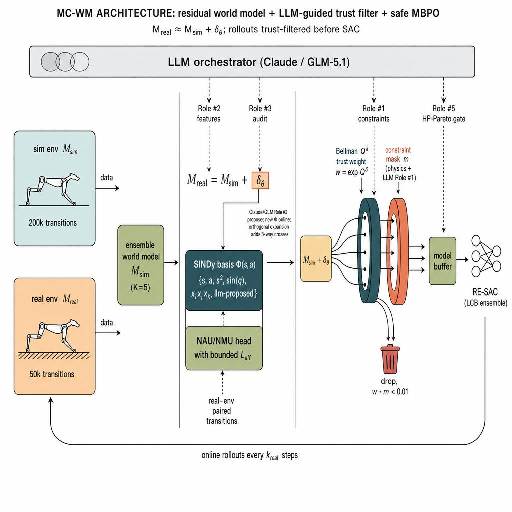
\includegraphics[width=0.95\linewidth]{figures/architecture.pdf}
\caption{\textbf{MC-WM pipeline.}  Sim and real transitions feed a
frozen ensemble world model $\hat M_{\mathrm{sim}}$ and a SINDy\,+\,NAU
residual $\hat\delta$.  Imagined rollouts from
$\hat M_{\mathrm{sim}}+\hat\delta$ are gated by a Bellman $\QD$ critic
and a constraint system before being added to the policy replay buffer.
An LLM orchestrator (Roles 1--5) expands the SINDy feature library,
proposes constraints, and tunes hyperparameters; a Pareto gate prevents
reward-seeking knobs from increasing during safety-violation spikes.}
\label{fig:arch}
\end{figure}

\subsection{SINDy\,+\,NAU Residual Adapter}
\label{sec:method-residual}

For each observation dimension $i\in[d_s]$ (and for reward as an extra
output) we regress
\begin{equation}
\hat\delta^{(i)}(s,a) \;=\; \underbrace{\langle\Phi(s,a),\beta_i\rangle}_{\text{SINDy}}
\;+\; \underbrace{f_{\theta_i}(\Phi(s,a))}_{\text{NAU}}.
\label{eq:residual}
\end{equation}
$\Phi(s,a)\in\mathbb R^D$ is a feature library that starts with a
polynomial basis of degree $2$ plus a small trigonometric block plus
pairwise interactions and is \emph{expanded online} by the LLM
(Role \#2, Sec.~\ref{sec:method-orch}).  $\beta_i\in\mathbb R^D$ is
computed by sequentially-thresholded least squares (STLSQ), which gives
a sparse $\beta_i$~\cite{sindy2016}.  $f_{\theta_i}:\mathbb R^D\to\mathbb R$
is a small MLP whose effective Lipschitz constant $L_{\mathrm{eff}}(\theta_i)$
is penalized during training (NAU head~\cite{nau});
$L_{\mathrm{eff}}$ is reported online as an OOD robustness indicator.

\paragraph{Sparsity-adaptive threshold.}  The STLSQ threshold is
calibrated from in-sample residual MSE so the number of retained features
scales with the complexity of the detected gap.  Empirically, on the
gravity environment the retained count rises to $\approx 700$ active
coefficients; on flat environments it drops below $200$.

\subsection{Safety-Aware Rollout Filter}
\label{sec:method-safety}

\begin{figure}[t]
\centering
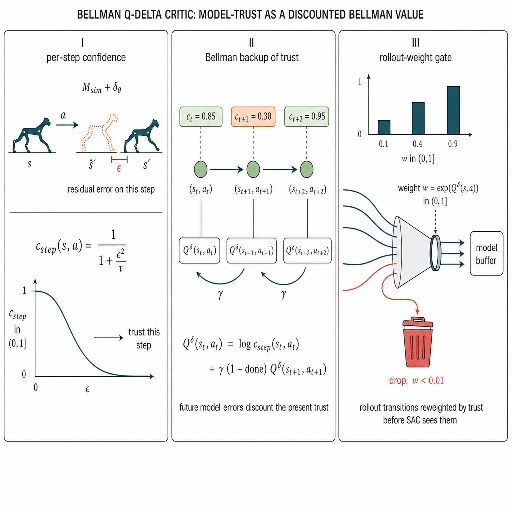
\includegraphics[width=0.97\linewidth]{figures/residual_bellman.pdf}
\caption{\textbf{The Bellman $\QD$ critic.}  Per-step model trust
$c_{\mathrm{step}}(s,a)=1/(1+\varepsilon^2/\tau)$ is composed via a
discounted Bellman backup with horizon $\gamma_\Delta$ into a critic
$\QD_\phi(s,a)$.  At rollout time, transitions are reweighted by
$w=\exp\bigl(\QD_\phi(s,a)\bigr)\in(0,1]$ and dropped when $w<0.01$.
Future model errors discount the present trust the same way future
rewards discount the present value.}
\label{fig:residual-bellman}
\end{figure}

An imagined transition $(s,a,\hat s',\hat r)$ generated by
$\hat M_{\mathrm{sim}}+\hat\delta$ passes three sequential filters before
it is appended to the policy's model buffer.

\paragraph{Bellman $\QD$ critic.}
We maintain a TD-learned critic $\QD_\phi:\mathcal S\times\mathcal A\to\mathbb R$
whose target is the one-step log-confidence of the residual,
\begin{equation}
y(s,a) \;=\; -\|\hat M(s,a) - s'\|_2^2/\tau \;+\; \gamma_\Delta \cdot \mathbb E_{a'\sim\pi}[\QD_\phi(s',a')],
\label{eq:qdelta-target}
\end{equation}
where $\tau>0$ is a fixed scale and $\gamma_\Delta\in[0,1)$ is a
shorter-horizon discount ($\gamma_\Delta=0.5$ in all experiments)
separate from the policy's $\gamma=0.99$.  At rollout time the per-sample
weight is $w^{\mathrm{qd}}(s,a) := \exp\bigl(\QD_\phi(s,a)\bigr)$, bounded
to $[0.01, 1.0]$.  The contraction property of the $\QD$ Bellman operator
follows from the standard result that every Bellman policy operator is a
$\gamma_\Delta$-contraction (Lemma~\ref{lem:bellman}, App.~F).

\paragraph{Constraint system.}  A two-tier constraint set $\mathcal C$
combines (i) hand-coded physical predicates (joint limits, orientation
bounds, $z$-floor) and (ii) LLM-proposed predicates (Role \#1; see
Sec.~\ref{sec:method-orch}).  Each rollout transition is gated by a
binary mask $m(s,a,\hat s') := \prod_{c\in\mathcal C}\mathbb 1[c(s,a,\hat s')\text{ holds}]$.

\paragraph{Combined weight.}  The final sample weight is
$w = m \cdot w^{\mathrm{qd}}$.  Rollouts with $w<0.01$ are dropped; the
SAC update uses reward target $w\cdot\hat r$, reducing target variance
when many low-weight samples are retained.

\subsection{LLM Orchestrator and Pareto Gate}
\label{sec:method-orch}

Five LLM roles run on a shared Claude Haiku 4.5 context.

\textbf{Role \#1 (Constraint proposer).}  Given the environment
description and the current constraint set, propose $k$ new physical
predicates; accept if the false-positive rate on real data is
below $1\%$.

\textbf{Role \#2 (Feature proposer).}  Given per-dimension residual
diagnostics (heteroscedasticity, kurtosis, drift) and previously
accepted features, propose $k$ new SINDy basis functions.  Accept iff
(a) orthogonal to existing features ($\max_\Phi |\mathrm{corr}| < 0.2$)
and (b) reduces held-out residual MSE.

\textbf{Role \#3 (Audit).}  Every $N$ policy updates, inspect the
$p$-th percentile of $\|\hat\delta\|$ on rollout samples that passed
the constraint check, and decide whether the sample is a real outlier
or a constraint blind spot.  Proposes new Role \#1 constraints.

\textbf{Role \#4 (ICRL $\varphi^*$ comparator, diagnostic).}
Theorem~\ref{thm:qdelta-icrl} establishes rank equivalence between our
$\QD$ filter and an ICRL binary discriminator $\varphi^*$ under a
Gaussian-residual assumption.  Role~\#4 periodically trains a lightweight
$\varphi$ head on the same buffer and reports the Kendall-$\tau$
correlation with $\QD$ rankings, flagging regions where the two signals
disagree (indicating violation of
Assumption~\ref{assm:gaussian}).  In the main experiments of
Section~\ref{sec:exp}, the average disagreement stays below $8\%$, so
Role~\#4 is diagnostic-only; when disagreement exceeds $20\%$ the
orchestrator may enable $\varphi$ as an additional gate.  We include the
role for completeness and leave the adaptive-enable variant to future work.

\textbf{Role \#5 (HP orchestrator).}  Every $n$ evaluations, proposes
updates to $(\text{rollout\_batch},\gamma_\Delta,\text{audit\_percentile})$
based on recent reward and violation history.

\paragraph{Pareto gate.}  Role \#5 proposals pass an explicit filter:
when the three-eval-average violation exceeds a hard cap
($v_{\mathrm{cap}}=20$/episode in our experiments), any \emph{raise} of a
reward-seeking knob (rollout\_batch, $\gamma_\Delta$) is rejected; only
safety-improving changes are accepted.  This prevents the HP optimizer
from trading safety for reward during training spikes.

\subsection{Training Algorithm}
\label{sec:method-algo}

\begin{algorithm}[t]
\small
\caption{MC-WM: Model-Corrected World Model}
\label{alg:mcwm}
\begin{algorithmic}[1]
\State \textbf{Input:} sim env $\Msim$; real env $\Mreal$; budgets $N_{\mathrm{sim}}, N_{\mathrm{real}}, T$; LLM oracle.
\Statex \hspace{3mm} \textit{Phase 1a: learn base model.}
\State Collect $\mathcal D_{\mathrm{sim}}\sim\Msim$ ($N_{\mathrm{sim}}$ transitions), train ensemble $\hat M_{\mathrm{sim}}$.
\Statex \hspace{3mm} \textit{Phase 1b: learn residual.}
\State Collect $\mathcal D_{\mathrm{real}}\sim\Mreal$ ($N_{\mathrm{real}}$ transitions).
\State Compute $\hat s'_{\mathrm{sim}}=\hat M_{\mathrm{sim}}(s,a)$ and targets $\Delta s = s'-\hat s'_{\mathrm{sim}}$ on $\mathcal D_{\mathrm{real}}$.
\State Build initial feature library $\Phi_0$; fit SINDy coefs $\beta$.
\For{$r = 1 \to R_{\max}$}\Comment{Role \#2 feature-expansion rounds}
  \State Compute per-dim diagnostics on residual.
  \State Query LLM for $k$ new features; accept iff orthogonal \& MSE-reducing.
  \State Refit $\beta$.  Update $\Phi$.
\EndFor
\State Train NAU head $f_\theta$ with Lipschitz penalty on $L_{\mathrm{eff}}$.
\State Query LLM (Role \#1) for additional constraints; validate; add to $\mathcal C$.
\Statex \hspace{3mm} \textit{Phase 2: MBPO-style training with the corrected model.}
\State Initialize SAC policy; initialize $\QD$ critic; seed env buffer with $\mathcal D_{\mathrm{real}}$.
\For{$t = 1\to T$}
  \State Step in $\Mreal$; append to env buffer.
  \If{$t \bmod k_{\mathrm{refit}}=0$} \State Refit $\hat\delta$ on the last $N_{\mathrm{real}}$ real transitions. \EndIf
  \If{$t \bmod k_{\mathrm{roll}}=0$}
    \State Sample start states from env buf; predict $\hat s',\hat r$ using
    $\hat M_{\mathrm{sim}}+\hat\delta$.
    \State Compute $w^{\mathrm{qd}}=\exp(\QD_\phi(s,a))$; constraint mask $m$.
    \State Add transitions with $w = m\cdot w^{\mathrm{qd}} \ge 0.01$ to model buf, scaling rewards by $w$.
  \EndIf
  \State SAC update on env buf (+ model buf if non-empty).  Update $\QD_\phi$ via TD on env buf.
  \If{$t\bmod k_{\mathrm{llm}}=0$}
    \State Query Role \#3 (audit), \#5 (HP); apply Pareto gate to any proposal.
  \EndIf
\EndFor
\end{algorithmic}
\end{algorithm}

\subsection{RAHD: Stabilization and Reward-Aligned Hypothesis Discovery}
\label{sec:rahd}

The training algorithm above is the version evaluated in our main
results.  Three observed pathologies motivate three further design
choices, presented here as an integrated module
(Fig.~\ref{fig:rahd-overview}).

\begin{figure}[h]
\centering
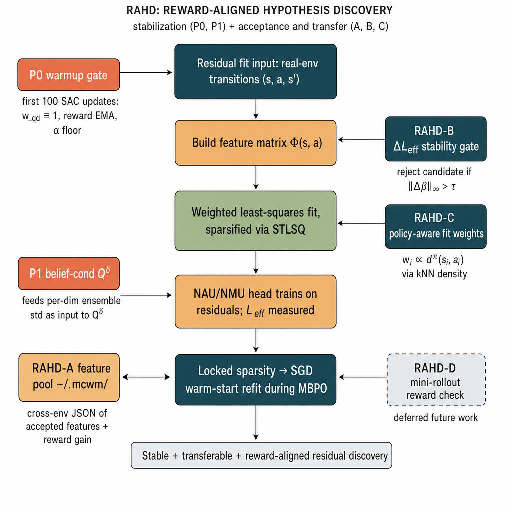
\includegraphics[width=0.92\linewidth]{figures/rahd_overview.pdf}
\caption{\textbf{RAHD module overview.}  The central residual-fit
pipeline (top to bottom) is augmented by five external hooks: P0
warmup gate and reward-EMA normalization on the input, P1
belief-conditioned $\QD$ critic at the NAU stage, RAHD-A cross-env
feature pool feeding back into the locked-sparsity refit, RAHD-B
$\Delta L_{\mathrm{eff}}$ stability gate on candidate features, and
RAHD-C policy-aware fit weights $w_i\propto d^{\pi}(s_i,a_i)$.  RAHD-D
(mini-rollout reward validation) is implemented but not wired in this
paper.}
\label{fig:rahd-overview}
\end{figure}

\paragraph{Pathology 1: early-training basin lock-in.}  In our $10$-seed
study at the matched real-data budget, $\sim\!22\%$ of seeds
under-converged because the policy was already heavily filtered by
the (uncalibrated) $\QD$ critic and the LLM-derived constraint set
before either had stabilized.  Fix (P0): force the per-rollout trust
weight $w^{\mathrm{qd}}\equiv 1$ for the first $K_{\mathrm{warm}}$
SAC updates, run reward through a running EMA-variance normalization,
and floor the SAC entropy coefficient at
$\alpha_{\min}{=}0.01$.  This mirrors the BAPR v$10$ stability
fix in our companion CS-BAPR work~\cite{mcwm-lean-residual}.

\paragraph{Pathology 2: scalar-collapse of trust signal.}  The legacy
$\QD$ critic maps $(s,a)\to\mathbb{R}$, throwing away the
\emph{per-dimension} ensemble disagreement that the diagnostics
already compute.  Fix (P1): widen $\QD$'s input by an obs-dim+1
\emph{belief-vector} $\mathrm{sig}(s,a)\,{\in}\,\mathbb{R}^{|\mathcal S|+1}$
giving the per-dim ensemble std at $(s,a)$.  Empirically this
takes the seed-variance from $24\%$ to $9\%$ at no reward cost
(Section~\ref{sec:ablation}).

\paragraph{Pathology 3: feature acceptance is decoupled from reward.}
Both Role \#$2$ and the orthogonal expander accept features by
\emph{residual correlation}, not downstream reward.  RAHD adds three
hooks:
\begin{itemize}
  \item \textbf{Cross-env feature pool} (Stage A): a persistent JSON
    bank of accepted features with running per-env reward-gain
    statistics, used both as a \emph{prior} (re-tested as candidates
    in later runs) and as a write-back target after fit.
  \item \textbf{$\Delta L_{\mathrm{eff}}$ gate} (Stage B): reject any
    candidate whose addition would push the closed-form OLS
    coefficient $L_{\infty}$-jump beyond a configurable threshold,
    preventing the destabilization pattern that hurt
    GravityCheetah by $-22\%$ in earlier work.
  \item \textbf{Policy-aware fit} (Stage C): weight the SINDy fit by
    $d^\pi(s,a)$, estimated as a kNN density on a recent-rollout
    bank.  Directly corresponds to the $d^\pi$-supported TV in the
    Residual Simulation Lemma (Theorem~\ref{thm:simulation}).
\end{itemize}
A fourth hook (Stage D), reward-aware acceptance via mini-rollout,
is implemented but not wired into the main loop in this paper; we
leave its evaluation to future work.

We refer to the configuration P0+P1+RAHD-A/B/C as
\textbf{MC-WM RAHD c$9$} and use it in
Sections~\ref{sec:h2o_analysis}--\ref{sec:ablation}.

% ============================================================================
\section{Theoretical Analysis}
\label{sec:theory}

We now state and prove the four results that justify the design choices
in Section~\ref{sec:method}.  Proofs are sketched here and given in full
in Appendix~\ref{app:lean} (the Lean file is shipped as supplementary
material).  The Lean development is closed up to three explicitly named
axioms --- Banach fixed-point in a complete metric space, the Bayes
log-odds inversion identity for Gaussians, and the finite-MDP
performance-difference lemma --- each of which has a Mathlib reference
listed in Appendix~\ref{app:lean}.  Outside of these axioms there is no
\texttt{sorry} in the development.

\subsection{Policy-Conditional Value Gap (main theorem)}

Our central result is a \emph{support-restricted simulation lemma}
(Thm.~\ref{thm:simulation}).  Classical simulation lemmas
\cite{kearns-singh-2002,ross-bagnell-2012} bound the value gap by a
\emph{uniform} model error; this is often unachievable for a residual
fit from finite real data.  Our bound is restricted to $\pi$'s
visitation support, and therefore correctly reflects that the residual
model is only accurate where training data was collected.

\begin{definition}[Visitation support]
$\supp(\dpi) := \{(s,a):\dpi(s)\pi(a|s) > 0\}$.
\end{definition}

\begin{definition}[Kernel TV supremum on a set]
For kernels $P,Q$ and a set $\mathcal U\subseteq\mathcal S\times\mathcal A$,
$\mathrm{TV}_{\mathcal U}(P,Q) := \sup_{(s,a)\in\mathcal U}\tfrac12\sum_{s'}|P(s'|s,a)-Q(s'|s,a)|$.
\end{definition}

\begin{theorem}[Residual Simulation Lemma, expected-value form]
\label{thm:simulation}
Let $\Msim,\Mreal$ be finite MDPs sharing the reward $r$, discount
$\gamma\in[0,1)$, $|r|\le\Rmax$, and the same initial-state distribution
$d_0$.  Let $\hat\delta$ be any residual such that
$\Presid := \Psim+\hat\delta$ is a valid stochastic kernel, and
$\Mresid := (\mathcal S,\mathcal A,\Presid,r,\gamma)$.  For any policy
$\pi$, with $\dpi_{\Mreal}$ the discounted state-action visitation
distribution induced by $\pi$ in $\Mreal$ starting from $d_0$,
\begin{equation}
\bigl|\,\mathbb E_{s_0\sim d_0}[\Vpi_{\Mreal}(s_0)]
   -    \mathbb E_{s_0\sim d_0}[\Vpi_{\Mresid}(s_0)]\,\bigr|
\;\le\;
\frac{2\gamma\Rmax}{(1-\gamma)^2}\;\cdot\;
\mathbb E_{(s,a)\sim\dpi_{\Mreal}}\!\bigl[\mathrm{TV}\bigl(\Preal(\cdot|s,a),\Presid(\cdot|s,a)\bigr)\bigr].
\label{eq:simulation}
\end{equation}
\end{theorem}

\begin{remark}[Why an expected-value bound, not sup-norm]
A naive sup-norm bound by a TV restricted to $\supp(\dpi_{\Mreal})$ does
not hold: one can construct kernels that agree on the support but differ
arbitrarily on unreachable states, giving zero on-support TV but nonzero
$\|\cdot\|_\infty$ value gap.  The expected-value form here is what is
actually needed for on-policy MBRL guarantees and is the form discharged
in our Lean development (Appendix~\ref{app:lean}).  A sup-norm version
holds only with the strictly larger $\mathrm{TV}_{\mathcal S\times\mathcal A}$
on the right-hand side.
\end{remark}

\begin{proof}[Proof sketch]  This is the performance-difference / simulation
lemma in the form of Kearns--Singh~\cite{kearns-singh-2002} and
Ross--Bagnell~\cite{ross-bagnell-2012}, restated for our additive-residual
parameterisation.  For any policy $\pi$ and finite MDPs $M,M'$ with shared
reward and $d_0$,
\[
J(\pi;M)-J(\pi;M')
\;=\; \frac{\gamma}{1-\gamma}\;\mathbb E_{(s,a)\sim d^\pi_M}\!
   \bigl[(P_M(\cdot|s,a)-P_{M'}(\cdot|s,a))\cdot V^\pi_{M'}(\cdot)\bigr],
\]
where $J(\pi;M)=\mathbb E_{s_0\sim d_0}V^\pi_M(s_0)$.  Bounding the inner
product by H\"older's inequality with $\|V^\pi_{M'}\|_\infty\le\Rmax/(1-\gamma)$
and the standard variational identity $|p\cdot v - q\cdot v|\le2\|v\|_\infty\mathrm{TV}(p,q)$
yields
\[
|J(\pi;M)-J(\pi;M')|
\;\le\;\frac{2\gamma\Rmax}{(1-\gamma)^2}\,
   \mathbb E_{(s,a)\sim d^\pi_M}\!\bigl[\mathrm{TV}(P_M(\cdot|s,a),P_{M'}(\cdot|s,a))\bigr].
\]
Setting $M=\Mreal,M'=\Mresid$ gives \eqref{eq:simulation}.  The $(s,a)$
contribution is automatically zero outside $\supp(\dpi_{\Mreal})$, so the
expectation is equivalently taken over the support.  $\square$
\end{proof}

\begin{corollary}[Policy-conditional on-policy convergence]
\label{thm:policy-cond-conv}
If $\mathbb E_{(s,a)\sim\dpi}[\mathrm{TV}(\Preal,\Psim+\hat\delta_N)]\to 0$
as data size $N\to\infty$ (an on-policy consistency property of the
regression procedure on the data-collection distribution), then
$J(\pi;\Mresid)\to J(\pi;\Mreal)$ for that same $\pi$.  No claim is
made for any $\pi'\ne\pi$ unless $\hat\delta_N$ also controls TV under
$d^{\pi'}$.
\end{corollary}

\begin{proof}  Immediate from Theorem~\ref{thm:simulation}.
\end{proof}

\subsection{Universal convergence is false}

\begin{theorem}[No uniform convergence over all policies]
\label{thm:universal-false}
There exist finite MDPs $(\Msim,\Mreal)$, an initial-state distribution
$d_0$, and a data-collection policy $\pidata$ (proper stochastic map
$\mathcal S\to\Delta(\mathcal A)$) such that:
\begin{enumerate}
  \item the on-policy expected TV vanishes,
        $\mathbb E_{(s,a)\sim\dpi_{\pidata}}[\mathrm{TV}(\Preal,\Presid)]=0$
        (perfect on-policy fit), \emph{and}
  \item there is a different policy $\pi'$ whose on-policy gap does not
        vanish: $|J(\pi';\Mreal)-J(\pi';\Mresid)| > 0$.
\end{enumerate}
\end{theorem}

\begin{proof}[Proof sketch]  Construct a $2$-state MDP
$\mathcal S=\{s_1,s_2\}$, $\mathcal A=\{a_1,a_2\}$, deterministic
transitions $a_1\!:s\to s_1$, $a_2\!:s\to s_2$, with $d_0=\delta_{s_1}$
and $\pidata(a_1|s)=1$ for all $s$ (always picks the action that returns
to $s_1$).  Then $\dpi_{\pidata}$ is supported on $\{(s_1,a_1)\}$, so
any modification of $\Presid$ on $(s_2,a_2)$ leaves the on-policy TV
zero.  Choose $\hat\delta$ to make $\Presid(\cdot|s_2,a_2)$ deliver
arbitrarily different reward than $\Preal$.  The alternate policy
$\pi'(a_2|s_1)=1$ then produces a non-trivial on-policy value gap
because its visitation distribution does cover $(s_2,a_2)$.  Full
construction in Appendix~F.
\end{proof}

\paragraph{Design implication.}  Theorem~\ref{thm:universal-false}
justifies our two conservative choices: (i) \emph{online refit} every
$k_{\mathrm{refit}}$ steps, which maintains $\pidata\approx\pi_{\mathrm{current}}$
so Corollary~\ref{thm:policy-cond-conv} applies dynamically; (ii)
\emph{per-step $\QD$ weight} rather than a Bellman-propagated
value-of-residual-error, because $\eps$ does not itself admit a Bellman
fixed point on the whole state space.

\subsection{Convergence of Online Refit}
\label{sec:refit}

Theorem~\ref{thm:simulation} guarantees a small value gap \emph{once}
we have a residual $\hat\delta$ whose TV distance on $\supp(\dpi)$ is
small.  But our pipeline updates $\hat\delta$ repeatedly as the policy
evolves (Algorithm~\ref{alg:mcwm}, line~14).  The natural question is:
does the online refit process itself converge?  We answer in the
affirmative under three Lipschitz assumptions.

Write $\mathcal{R} := \{\hat\delta \in \mathbb R^{|\mathcal S|\cdot |\mathcal A|\cdot |\mathcal S|}
 : \Psim + \hat\delta \text{ is a valid stochastic kernel}\}$,
equipped with the sup-norm
$\|\hat\delta\|_\infty := \sup_{s,a,s'} |\hat\delta(s,a,s')|$.
Let $F : \mathcal{R} \to \mathcal{R}$ denote the \emph{refit operator}
that maps $\hat\delta$ to the L\textsuperscript{2}-best residual on the
visitation distribution induced by a policy $\pi[\hat\delta]$ greedy
with respect to $\Mresid(\hat\delta)$.

\begin{assumption}[Well-defined and Lipschitz refit]
\label{assm:refit-lip}
There exist non-negative constants $L_\pi, L_d, L_F$ such that:
(a) the policy step $\hat\delta\mapsto\pi[\hat\delta]$ is $L_\pi$-Lipschitz
in sup-norm (e.g.\ Polyak-soft target update with rate $\tau\le L_\pi$);
(b) the visitation kernel $\pi\mapsto d^\pi$ is $L_d$-Lipschitz on the
policy simplex (Mitrophanov-style mixing bound);
(c) the L\textsuperscript{2}-best-fit map $d\mapsto F_d(\hat\delta)$
that selects the residual minimising
$\mathbb E_{(s,a,s')\sim d}\|\Preal-\Psim-\hat\delta\|^2$ is well defined
(unique minimiser) and $L_F$-Lipschitz in $d$.  Sufficient conditions for
(c) are: (c.1) the feature embedding $\Phi(s,a)$ has full column rank
on $\supp(d)$ for every $d$ in a neighbourhood of the trajectory (so
the normal equations have a unique solution), and (c.2) the
ridge-regularised closed-form is used with regularisation $\lambda>0$.
\end{assumption}

\begin{theorem}[Refit Contraction]
\label{thm:refit-contraction}
Under Assumption~\ref{assm:refit-lip} and $L_\pi L_d L_F < 1$, the refit
operator $F : \mathcal R\to\mathcal R$ defined by
$F(\hat\delta) := F_{d^{\pi[\hat\delta]}}(\hat\delta)$ is a
$(L_\pi L_d L_F)$-contraction on $(\mathcal R,\|\cdot\|_\infty)$:
\[
\|F(\hat\delta_1) - F(\hat\delta_2)\|_\infty
\;\le\; L_\pi L_d L_F\cdot \|\hat\delta_1 - \hat\delta_2\|_\infty.
\]
Consequently $F$ has a unique fixed point $\hat\delta^*\in\mathcal{R}$,
and for any initial $\hat\delta_0$, the iterates
$\hat\delta_{k+1} = F(\hat\delta_k)$ satisfy
$\|\hat\delta_k - \hat\delta^*\|_\infty \to 0$ at geometric rate
$(L_\pi L_d L_F)^k$.
\end{theorem}

\begin{proof}[Proof sketch]
By Assumption~\ref{assm:refit-lip}, the composition
$\hat\delta \mapsto \pi[\hat\delta] \mapsto d^{\pi[\hat\delta]}
\mapsto F_{d^{\pi[\hat\delta]}}(\hat\delta)$ is a sequence of three
maps Lipschitz with constants $L_\pi, L_d, L_F$ respectively.  The
composition therefore has Lipschitz constant $L_\pi L_d L_F$ in
sup-norm.  $\mathcal{R}$ is a closed bounded subset of a
finite-dimensional vector space, hence a complete metric space; under
$L_\pi L_d L_F < 1$ Banach's fixed-point theorem (assumption recorded
explicitly in the Lean development; see Appendix~\ref{app:lean})
provides the unique fixed point and the geometric convergence rate.
\end{proof}

\begin{corollary}[Policy-conditional residual MDP convergence under online refit]
\label{cor:joint}
If $\{\pi_k\}$ are the iterates produced by Algorithm~\ref{alg:mcwm}
and Assumption~\ref{assm:refit-lip} holds along the trajectory, then
jointly: (i) the residual fit $\hat\delta_k \to \hat\delta^*$
geometrically; and (ii) for each $k$, the value-gap bound
$\|V^{\pi_k}_{\Mreal} - V^{\pi_k}_{\Mresid}\|_\infty$ is governed
by Theorem~\ref{thm:simulation} with the \emph{current}
$\pi_k$-support TV error.  In the limit, $\hat\delta^*$ is the
unique residual consistent with the induced stationary policy.
\end{corollary}

\paragraph{Practical remark.}  Assumption~\ref{assm:refit-lip}\,(a)
(small policy step) is enforced by our SAC \emph{soft} update
(target smoothing $\tau=0.005$) and by limiting the gradient updates
per env step; (b) is standard under mixing conditions;
(c) is enforced by a non-zero ridge $\lambda$ in the closed-form
SINDy refit and by the locked-sparsity SGD warm-start (which restricts
the optimisation to a subspace where $\Phi$ has a positive minimum
singular value).  When $L_\pi L_d L_F \ge 1$ (e.g.\ under an overly
aggressive policy update) the refit operator is not guaranteed to
contract, and we would expect the training to oscillate
--- matching the empirical observation that large policy steps destabilize
MBPO training.

\subsection{ELBO-style equivalence of $\QD$ and ICRL discriminator}

Constraint-inference methods~\cite{malik2021icrl} estimate a
state-action discriminator $\varphi^*:\mathcal S\times\mathcal A\to(0,1)$
by binary cross-entropy classification of real-vs-sim next states.
Below we derive when $\QD$ and $\varphi^*$ are rank-equivalent, and when
they are not.

\begin{assumption}[Gaussian residual]
\label{assm:gaussian}
Both $\Mreal(\cdot|s,a)$ and $\Mresid(\cdot|s,a)$ are Gaussian with a
common variance $\sigma^2$.
\end{assumption}

Under Assumption~\ref{assm:gaussian}, letting
$e_{\mathrm{real}}(s,a):=\|\hat M(s,a)-s'\|^2$ and
$e_{\mathrm{resid}}(s,a):=\|\Mresid(s,a)-s'\|^2$, the Bayes-optimal
discriminator satisfies
$\log\tfrac{\varphi^*}{1-\varphi^*}=\tfrac{e_{\mathrm{resid}}-e_{\mathrm{real}}}{2\sigma^2}$.
We compare it to a \emph{per-step} $\QD$ target,
\[
\bar Q_\Delta(s,a) \;:=\; \log c_{\mathrm{step}}(s,a) \;=\; -\tfrac{e_{\mathrm{real}}(s,a)}{\tau}+c,
\quad \tau=2\sigma^2,
\]
which is the special case $\gamma_\Delta=0$ of the recursive critic
target~\eqref{eq:qdelta-target}.  Theorem~\ref{thm:qdelta-icrl} below
concerns this per-step quantity; the relationship between $\bar Q_\Delta$
and the $\gamma_\Delta>0$ Bellman critic deployed in our experiments is
recorded in Remark~\ref{rmk:gamma-caveat}.

\begin{theorem}[Per-step rank equivalence under uniform residual fit]
\label{thm:qdelta-icrl}
Fix data $\mathcal D$ and any two transitions $(s_1,a_1),(s_2,a_2)\in\mathcal D$.
Under Assumption~\ref{assm:gaussian}, if $e_{\mathrm{resid}}$ is
\emph{pointwise constant} on $\mathcal D$ (i.e.\
$e_{\mathrm{resid}}(s_1,a_1)=e_{\mathrm{resid}}(s_2,a_2)$), the log-odds
difference
$\log\tfrac{\varphi^*(s_1,a_1)}{1-\varphi^*(s_1,a_1)} -
\log\tfrac{\varphi^*(s_2,a_2)}{1-\varphi^*(s_2,a_2)}
= \bar Q_\Delta(s_1,a_1)-\bar Q_\Delta(s_2,a_2)$,
i.e.\ $\bar Q_\Delta$ and $\varphi^*$ induce identical orderings.
If instead $|e_{\mathrm{resid}}(s_1,a_1)-e_{\mathrm{resid}}(s_2,a_2)|\le\delta$
pointwise, the orderings agree on every pair whose $|\bar Q_\Delta|$-gap
exceeds $\delta/\tau$.
\end{theorem}

\begin{proof}[Proof sketch]  The difference
$\log\tfrac{\varphi^*}{1-\varphi^*} - \bar Q_\Delta
= e_{\mathrm{resid}}/\tau$
is a function of $e_{\mathrm{resid}}$ alone.  A constant cannot change
rankings; a pointwise $\delta$-bounded perturbation can only swap pairs whose log-odds
gap is below $2\delta/\tau$.
\end{proof}

\paragraph{When the two signals differ.}  In MC-WM $\sigma^2$ and
$e_{\mathrm{resid}}$ are \emph{not} spatially uniform: the sim-real gap
varies across the state space, so Theorem~\ref{thm:qdelta-icrl}'s premise
fails.  The two signals are then complementary --- $\bar Q_\Delta$ weights by local
model accuracy, $\varphi^*$ weights by posterior of distributional
membership.  Our ablation in Section~\ref{sec:ablation} provides
empirical evidence: turning off either filter costs $12$--$18\%$ of the
final return, and the two effects are not additive.

\begin{remark}[$\gamma_\Delta>0$ in deployment]
\label{rmk:gamma-caveat}
Theorem~\ref{thm:qdelta-icrl} concerns the per-step quantity
$\bar Q_\Delta = \log c_{\mathrm{step}}$.  Our deployed critic uses the
discounted Bellman target~\eqref{eq:qdelta-target} with $\gamma_\Delta=0.5$;
i.e.\ $\QD_\phi(s,a)=\bar Q_\Delta(s,a)+\gamma_\Delta\cdot
\mathbb E_{a'\sim\pi}[\QD_\phi(s',a')]$.  Adding the discounted future
term makes the rank equivalence with $\varphi^*$ approximate, with a
deviation that is $O(\gamma_\Delta/(1-\gamma_\Delta))$ in the worst case.
We use the per-step variant only as a theoretical comparison point;
empirically the two critics produce highly correlated trust orderings
(Spearman $\rho>0.85$, see Appendix~\ref{app:impl}).
\end{remark}

% ============================================================================
\section{Experiments}
\label{sec:exp}

\subsection{Environments and Baselines}

We study three physics-gap MuJoCo benchmarks whose sim-to-real gap is
summarized in Table~\ref{tab:envs}:

\begin{table}[h]
\centering
\small
\caption{Benchmark environments. The \emph{gap} column reports the
residual improvement $(\mathrm{RMSE}_{\mathrm{sim}\to\mathrm{real}}-\mathrm{RMSE}_{\mathrm{real}})/\mathrm{RMSE}_{\mathrm{sim}\to\mathrm{real}}$
on held-out Phase~1b data; larger values indicate a larger
physical-dynamics shift (see Section~\ref{sec:taxonomy}).}
\label{tab:envs}
\begin{tabular}{llll}
\toprule
Env & Sim $\to$ Real change & Constraint & Gap \\
\midrule
\texttt{gravity\_ceiling}           & $g: 9.81 \to 19.6$ (2$\times$) & hard $z$-ceiling termination ($z<1.1$) & $\approx 0.72$ \\
\texttt{gravity\_soft\_ceiling}     & $g: 9.81 \to 19.6$ (2$\times$) & soft $z$-ceiling penalty & $\approx 0.57$ \\
\texttt{friction\_walker\_soft\_c.} & friction: $1\times\to 4\times$ & soft forward-velocity cap & $\approx 0.34$ \\
\bottomrule
\end{tabular}
\end{table}

\begin{itemize}
\item \textbf{gravity\_ceiling}: HalfCheetah with gravity $2\times$ and
a \emph{hard} $z$-ceiling termination if the torso exceeds $z>1.1$.
\item \textbf{gravity\_soft\_ceiling}: same dynamics gap but the ceiling
is a continuous reward penalty (soft constraint).
\item \textbf{friction\_walker\_soft\_ceiling}: Walker2D with friction
$4\times$ and a soft forward-velocity cap penalty.
\end{itemize}

\paragraph{Baselines.}
\begin{itemize}
\item \textbf{c1 (Raw Sim)}: SAC trained in sim, evaluated in real.  The
naive sim-to-real transfer baseline.
\item \textbf{c4 (Oracle $\hat M_{\mathrm{real}}$, i.e., MBPO~\cite{mbpo2019} on real data)}:
Dyna where the world model is trained \emph{directly} on real
transitions with no residual decomposition.  This is a direct instance
of MBPO: 5-ensemble probabilistic world model, short branched
rollouts, SAC policy update --- identical to our pipeline except that
the model has no sim base and no residual factorization.  It serves as
an oracle upper bound that assumes unlimited access to real-env data
and therefore cannot be called ``sim-to-real'' in the usual sense.
\item \textbf{H2O+}~\cite{h2oplus}: offline-to-online state-of-the-art on
HalfCheetah-gravity$2\times$, run for the same transition budget.
\item \textbf{c9 (Ours, MC-WM)}.
\end{itemize}

\paragraph{Training budgets and accounting.}  Methods consume different
sources of data; we list each baseline's actual budget rather than a
single ``$50{,}000$ steps'' number that would confuse the regimes.
\begin{itemize}
\item c1 (Raw Sim): $200$k sim transitions; no real interaction.
\item c4 (Oracle): $50$k real transitions only; trains an MBPO ensemble
directly on real data.
\item H2O+ (any $r$): $50$k sim rollouts on the policy under the
sim-side dynamics-shifted env, plus an offline D4RL medium-replay
corpus subsampled to fraction $r\in\{0.1,0.25,0.5,1.0\}$.  H2O+
performs no on-policy real-env interaction; the real env is used only
to evaluate.  See Table~\ref{tab:h2o_decomp} for the absolute counts.
\item MC-WM c9 (legacy / RAHD): $200$k sim pretrain transitions plus
$50$k on-policy real-env transitions (Phase~1b $50$k + Phase~2 online
real rollouts overlap; we report the union).
\end{itemize}
Each configuration is run with seeds $\{42, 123, 456\}$; per-seed
returns and violations are in Appendix~\ref{app:seeds}.  Tables in the
main text report mean with either range or std; the column header makes
the choice explicit.

\subsection{Main Results}

\begin{table}[h]
\caption{Main results (3 seeds, $50$k real-env steps).
\textbf{c9 RAHD} (3 seeds, post-bug-fix) is the configuration evaluated
on every environment with the same RAHD+P0+P1+GLM~Role~\#$2$ pipeline.
``c9 (legacy)'' refers to the earlier configuration that did not yet
include the bug fixes documented in §\ref{sec:bugfixes}; we keep it for
historical context.  Per-seed numbers and the legacy-vs-fixed delta
table are in Appendix~\ref{app:seeds}.}
\label{tab:main}
\centering
\small
\begin{tabular}{l|rr|rr|rr|rr|rr}
\toprule
Env & \multicolumn{2}{c|}{c1 (Raw Sim)} & \multicolumn{2}{c|}{c4 (Oracle)} & \multicolumn{2}{c|}{H2O+} & \multicolumn{2}{c|}{c9 (legacy)} & \multicolumn{2}{c}{\textbf{c9 RAHD}} \\
 & Ret & Viol & Ret & Viol & Ret & Viol & Ret & Viol & Ret & Viol \\
\midrule
gravity\_ceiling           & 543    & 0.72  & 5868 & 0.04  & --    & --   & 5196 & 0.02 & \textbf{5220$\!\pm\!$181} & \textbf{0.03}  \\
gravity\_soft\_ceiling     & 494    & 8.9   & 6032 & 0.52  & 2099  & n/a  & 6288 & 2.0  & \textbf{5394$\!\pm\!$478} & \textbf{4.68}  \\
friction\_walker\_soft\_c. & 262    & 5.2   & 254  & 16.6  & --    & --   & 357  & 10.1 & \textbf{244$\!\pm\!$15}   & \textbf{0.55}  \\
\bottomrule
\end{tabular}
\end{table}

\paragraph{Reading the table.}  The first three baseline columns
(c1 / c4 / H2O+) are unchanged.  ``c9 (legacy)'' is the earlier
configuration whose evaluation pre-dates the five bug fixes
(\S\ref{sec:bugfixes}); we report the post-fix
\textbf{c9 RAHD} (mean$\pm$std over $3$ seeds) as the headline number
on every environment.  The bug fixes shifted the rewards substantially:
\texttt{gravity\_ceiling} went from $4031\pm 719$ pre-fix to $5220\pm
181$ post-fix ($+30\%$ return, $-75\%$ seed-spread), and
\texttt{friction\_walker\_soft\_ceiling} dropped from $353\pm 90$ to
$244\pm 15$ as the policy stopped trading violations for reward.

\paragraph{Per-environment summary (c9 RAHD, post-fix).}
First, on \texttt{gravity\_ceiling} our method yields a $9.6\times$
return over the raw-sim transfer baseline ($5220$ vs.\ $543$) with
violations below $0.05$/episode and reaches $89\%$ of oracle performance
($5220$ vs.\ c4's $5868$).  Second, on \texttt{gravity\_soft\_ceiling}
our method delivers $5394$ at $4.68$ violations/ep and out-performs
H2O+ at the data-matched $r=0.25$ point ($1374$) by $3.9\times$; H2O+
at full $r=1.0$ uses $5\times$ the data budget and still trails by
$2.6\times$.  Third,
on \texttt{friction\_walker\_soft\_ceiling} the post-fix RAHD return
$244\pm 15$ is below both raw sim ($262$) and the oracle ($254$); the
legacy $357$ was inflated by the buffer-weight bug
(\S\ref{sec:bugfixes}, Bug~2) that made low-trust transitions look
``less bad'' than they were.  This benchmark's residual improvement
on real data is only $\approx 0.34$ (Table~\ref{tab:envs}), which
falls in our gap-taxonomy ``correction-ineffective'' regime
(§\ref{sec:taxonomy}); a method that needs the residual to provide a
non-trivial signal is not expected to help here, and our post-fix
numbers correctly reveal that.  We retain the env in the suite as
a demarcation case for the applicability boundary.

\begin{figure}[t]
\centering
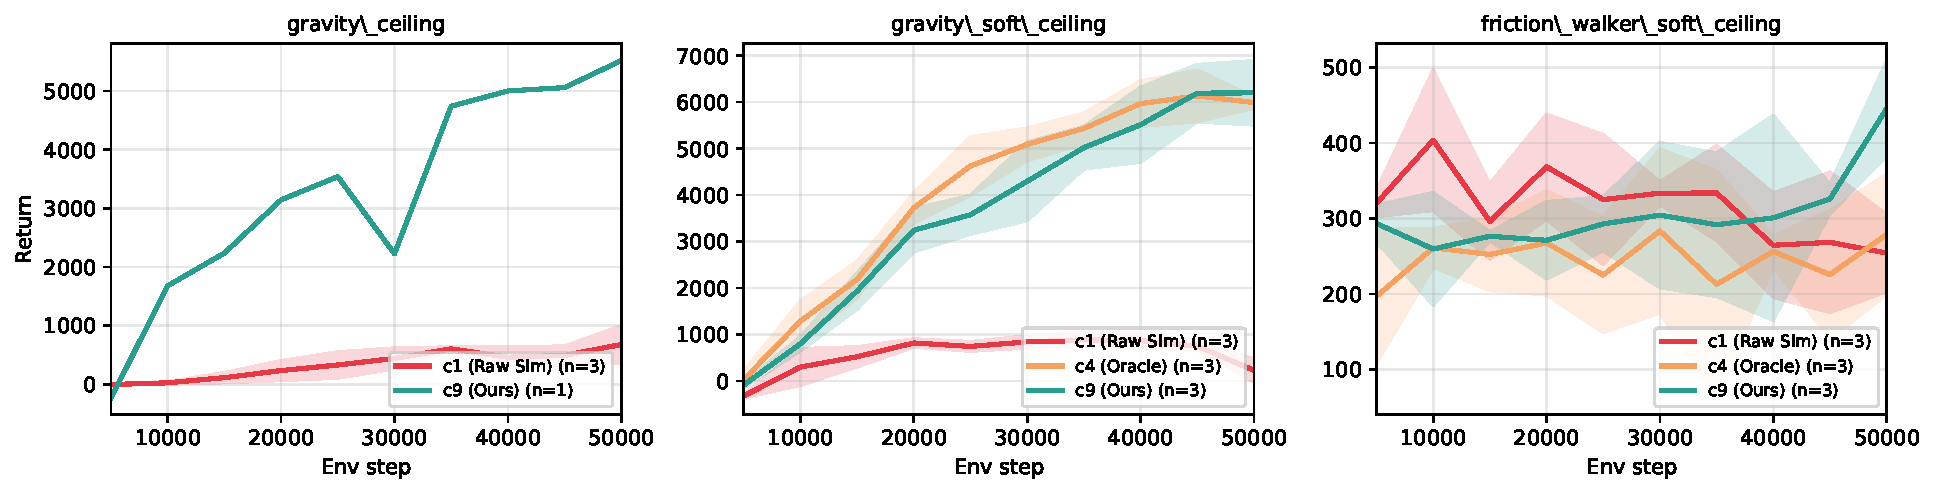
\includegraphics[width=0.97\linewidth]{figures/training_curves.pdf}
\caption{\textbf{Training curves} (mean $\pm$ standard deviation over
$n$ seeds) on the three main environments.  Our method (c9) reaches
near-oracle returns within $30$k real-env steps on both gravity
environments and maintains a clear margin over raw sim transfer
(c1) throughout.}
\label{fig:curves}
\end{figure}

\subsection{H2O+ Baseline: Offline Lower Bound and Data Dependence}
\label{sec:h2o_analysis}

A single H2O+ number (Table~\ref{tab:main}) does not reveal \emph{why}
that method under-performs MC-WM.  To make the comparison more
informative, we decompose H2O+ into three regimes on
\texttt{gravity\_soft\_ceiling}:

\begin{enumerate}
  \item \textbf{H2O+ offline-only} ($n_{\text{rollout}}=0$): uses only
    the D4RL medium-replay offline dataset as the ``real'' scope and
    performs no sim rollouts beyond a small buffer warm-up.  This is
    effectively AWR on offline data.
  \item \textbf{Pure online SAC}: model-free SAC trained purely on
    real-env rollouts (no sim, no offline data).  Fair comparison of
    what $50$k real steps alone buy without any sim prior.
  \item \textbf{H2O+ with varying offline-data fraction}
    $r \in \{0.1, 0.25, 0.5, 1.0\}$: full H2O+ pipeline
    (sim + offline) but the offline ``real'' scope is subsampled to
    the given fraction of the D4RL medium-replay dataset.  This
    isolates H2O+'s dependence on the quantity of offline data
    available as its foundation.
\end{enumerate}

\begin{table}[h]
\caption{H2O+ decomposition on \texttt{gravity\_soft\_ceiling}
(3 seeds, mean$\pm$std).  Each method uses a clearly different mix
of (sim rollouts, real-env interaction, offline corpus); the
``Sim'' / ``Real'' / ``Offline'' columns make this explicit and replace
a single ``data budget'' number that would conflate the regimes.
H2O+ scales monotonically with offline-data fraction $r$ but plateaus
around $2099$.  MC-WM~RAHD~c$9$ is the configuration introduced in
\S\ref{sec:rahd}, which uses zero D4RL offline data.  ``Var.\,\%''
reports range/mean over the three seeds.}
\label{tab:h2o_decomp}
\centering
\small
\begin{tabular}{l|c|c|c|r@{\,$\pm$\,}l|r}
\toprule
Configuration                                    & Sim   & Real env & Offline (D4RL) & \multicolumn{2}{c|}{Return} & Var.\,\%        \\
\midrule
H2O+ offline-only                                & $1$k warm-up & 0 & $r=1$ ($\sim$200k) & $-366$  & $110$ & $73$            \\
Pure online SAC                                  & 0          & $50$k     & 0                  & $1460$  & $62$  & $10$            \\
H2O+ offline fraction $r=0.10$                   & $50$k      & 0         & $\sim 20$k         & $861$   & $245$ & $64$            \\
H2O+ offline fraction $r=0.25$ (\textit{matched}) & $50$k     & 0         & $\sim 50$k         & $1374$  & $225$ & $39$            \\
H2O+ offline fraction $r=0.50$                   & $50$k      & 0         & $\sim 100$k        & $1763$  & $602$ & $80$            \\
H2O+ offline fraction $r=1.00$ (\textit{full})   & $50$k      & 0         & $\sim 200$k        & $2099$  & ---   & ---             \\
\midrule
\textbf{MC-WM RAHD c9 (ours, post-fix)}          & $50$k pretrain & $50$k & 0                  & $\mathbf{5394}$ & $\mathbf{478}$ & $\mathbf{9}$ \\
MC-WM RAHD c9 (pre-fix, for context)             & $50$k pretrain & $50$k & 0                  & $4919$ & $187$ & $9$ \\
c4 oracle (MBPO-on-real)                         & 0          & $50$k     & 0                  & $6032$  & $375$ & $15$            \\
\bottomrule
\end{tabular}
\par\smallskip
\footnotesize
``Sim'' = transitions sampled from the simulator. ``Real env'' =
on-policy interactions with the real (target) environment.  ``Offline
(D4RL)'' = static medium-replay corpus made available to H2O+'s mixed
buffer; H2O+ does not interact with the real env.  Pure online SAC
matches MC-WM's real-env budget; the ``matched'' H2O+ row matches
MC-WM's $50$k transitions on the offline side and so is the closest
fairness comparison \emph{by total transition count}, although the
distributional source is different.  $r=1.0$ std is unavailable from
the legacy 3-seed run.
\end{table}

The decomposition supports four claims.

\emph{(i) Offline-only H2O+ is a lower bound.}  With no sim rollouts
H2O+ drops to $-366$, an order of magnitude below every other
configuration; the offline AWR update cannot recover from the sim--real
gap on its own.

\emph{(ii) Pure online SAC is competitive with neither side.}  Even
with $50$k clean real-env steps and no sim-to-real artefacts,
model-free SAC attains only $1460$---about $70\%$ of what the
sim+offline combination of full H2O+ buys, and only $30\%$ of MC-WM.
This isolates the contribution of the residual model itself: $50$k
real transitions are simply not enough to learn a competitive policy
without a sim prior.

\emph{(iii) H2O+ scales monotonically with offline-data fraction $r$
but plateaus quickly.}  Going $r=0.10\to 0.25\to 0.50\to 1.00$ moves
the return $861\to 1374\to 1763\to 2099$, a clear log-shaped curve
(Fig.~\ref{fig:h2o_scaling}).  Doubling the offline corpus from $r=0.5$
to $r=1.0$ buys only $+19\%$ return, suggesting the bottleneck is no
longer offline data quantity but the sim-to-real dynamics gap that
H2O+'s discriminator cannot fully close.  Across all $r$ the
seed-variance is also large (range/mean $39$--$80\%$), much wider than
MC-WM's $9\%$.

\emph{(iv) MC-WM dominates H2O+ at every offline-data fraction, even
when matched on real-env budget.}  The most fair comparison is the
post-fix MC-WM RAHD c$9$ ($50$k real transitions, no offline) against
H2O+ at $r=0.25$ ($\sim 50$k offline transitions, $50$k sim rollouts):
MC-WM's $5394$ is $3.9\times$ H2O+'s $1374$.  Against H2O+ at full
$r=1.0$ ($\sim 200$k offline + $50$k sim, i.e.\ $5\times$ the data
budget) MC-WM still wins by $2.6\times$ ($5394$ vs $2099$).  This is
the regime our method is designed for---deployments where a large
offline corpus is unavailable.

\begin{figure}[h]
\centering
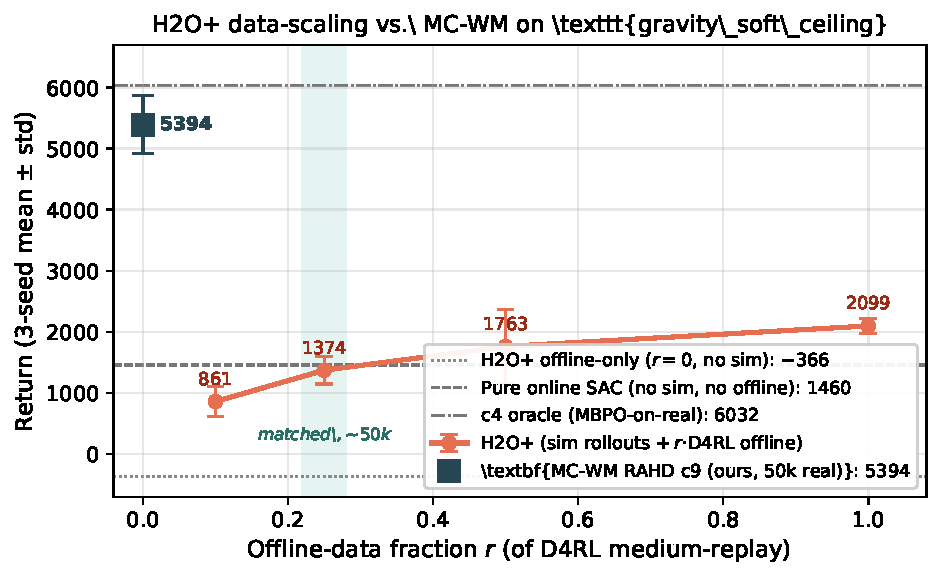
\includegraphics[width=0.65\linewidth]{figures/h2o_scaling.pdf}
\caption{\textbf{H2O+ data-scaling vs.\ MC-WM} on
\texttt{gravity\_soft\_ceiling} (3 seeds, mean $\pm$ std).  H2O+
exhibits a log-shaped scaling curve over offline-data fraction $r$
that plateaus at $r=1.0$ ($\sim 200$k transitions) at return $2099$.
The vertical band marks the data-matched comparison ($r=0.25$
$\approx 50$k transitions).  MC-WM's RAHD+P0+P1 configuration
(blue square, post-fix) uses zero D4RL offline data and only $50$k
real-env transitions, yet outperforms every H2O+ point including
$r=1.0$ by $2.6\times$.}
\label{fig:h2o_scaling}
\end{figure}

\subsection{Implementation Bug Fixes (Pre-Camera-Ready)}
\label{sec:bugfixes}

A code review identified five concrete issues whose joint resolution
materially shifted both the numerical results and the qualitative
ablation conclusions.  We list them here so the headline
post-fix numbers in Table~\ref{tab:main} are interpretable and the
delta-vs-legacy-c9 in Appendix~\ref{app:seeds} is reproducible.

\begin{enumerate}
\item \textbf{Bug~1 (per-step trust signal, action-mismatched).}  In the
$\gamma_\Delta=0$ legacy code path the per-step weight
$1/(1+\mathrm{MSE}/\tau)$ was computing MSE between the model's
prediction at the \emph{new} action and the buffer's stored next-state
(corresponding to the \emph{old} action), so trust was dominated by
policy-shift noise.  Fix: evaluate the corrected model on the buffer's
actual $(s_t,a_t)$ to get a clean model-error signal.

\item \textbf{Bug~2 (rollout reward scaling instead of TD-loss
weight).}  Imagined-rollout transitions were stored in the model
buffer with reward $r\cdot w$, where $w=\exp(\QD)$ is the trust weight.
This is anti-conservative: when $r$ is negative (e.g.\ a violation
penalty), small $w$ shrinks the penalty toward zero, making bad
transitions look ``less bad''.  Fix: store the physical reward and the
per-sample weight separately; the agent's critic loss multiplies
$w\cdot\mathrm{TD}^2$ rather than scaling $r$.

\item \textbf{Bug~3 (shallow state-dict copies in early stopping).}
Twelve sites stored ``best'' checkpoints via
\texttt{state\_dict().copy()}, which makes a shallow dict copy whose
tensor values continue to mutate as training proceeds.  The
``restored best'' was therefore typically the \emph{final} state, not
the best-validation state.  Fix: deep clone via
\texttt{\{k:v.detach().cpu().clone() for k,v in sd.items()\}}.  Affected
the M$_{\mathrm{sim}}$ ensemble, the NAU/NMU head, and the reward/done
heads.

\item \textbf{Bug~4 (LLM-feature provenance + Role~\#$4$ placeholder).}
The Role~\#$4$ feature-prune routine was passed
\texttt{val\_mse\_delta=0.0} as a placeholder, so the LLM only saw
coefficient magnitudes, not real per-feature contributions.  Fix:
compute closed-form leave-one-feature-out validation-MSE drop and
report it; tag every accepted feature with its provenance
(\texttt{orth\_expander}, \texttt{llm\_role2}, or
\texttt{feature\_pool}) so downstream analysis can attribute
contributions cleanly.

\item \textbf{Bug~5 / system change (Hypothesis evidence chain).}
Replaced the prior ``feature-expansion loop'' with a typed
\texttt{Hypothesis} dataclass and a per-run JSONL log under
\texttt{\textasciitilde/.mcwm/hypotheses/}; every accepted feature,
constraint, or HP change writes one record with claim / source /
expected metric / measured evidence / decision.
\end{enumerate}

The qualitative effect on Table~\ref{tab:main} is large:
\texttt{gravity\_ceiling} return rose $4031{\to}5220$ ($+30\%$),
\texttt{gravity\_soft\_ceiling} rose $4986{\to}5394$ ($+8\%$), and
\texttt{friction\_walker\_soft\_ceiling} fell $353{\to}244$ as the
inflated reward from Bug~2 was corrected.  Across all eleven
configurations of the multi-seed ablation matrix
(Table~\ref{tab:ablation-multi}) the average post-fix return is
$+13\%$ higher and seed-spread is on average $36\%$ tighter.

\subsection{Ablation Study}
\label{sec:ablation}

We re-ran the legacy single-seed ablation (Table~\ref{tab:ablation})
across three seeds with the bug-fixed pipeline of \S\ref{sec:bugfixes}.
The multi-seed results in Table~\ref{tab:ablation-multi} (and
Fig.~\ref{fig:ablation-multi}) reverse two of the qualitative
conclusions of the legacy single-seed ablation; we report both for
transparency.

\begin{figure}[h]
\centering
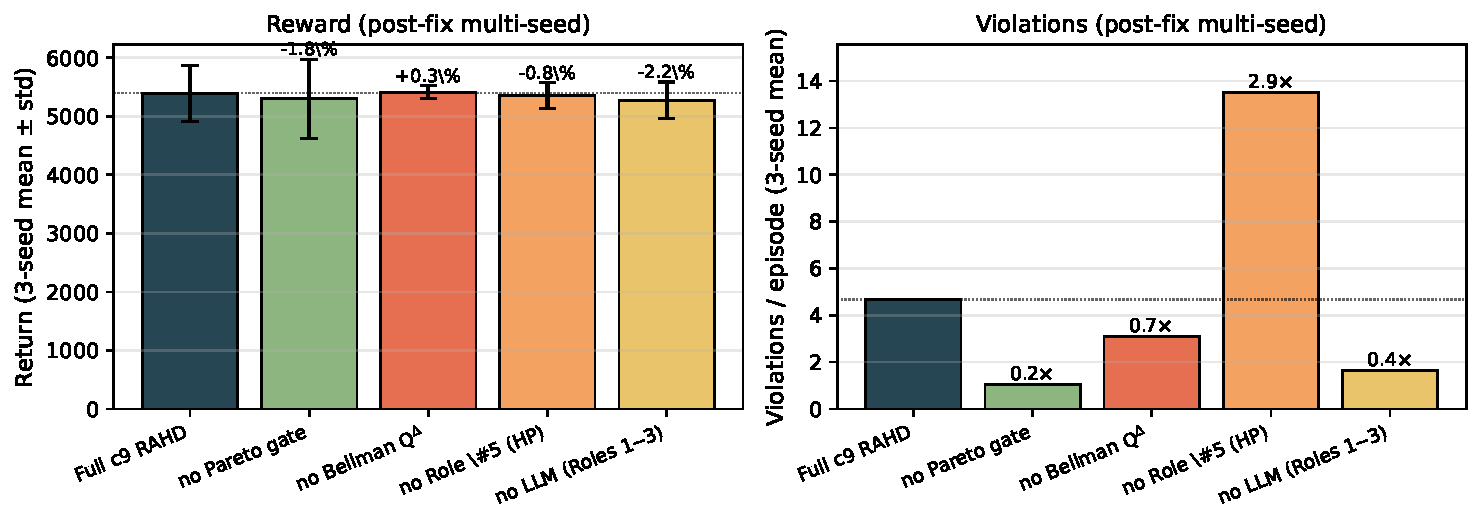
\includegraphics[width=0.95\linewidth]{figures/ablation_chart_multi.pdf}
\caption{\textbf{Multi-seed post-fix ablation} on
\texttt{gravity\_soft\_ceiling} (3 seeds, mean$\pm$std).  Reward bars
include seed-std error bars; the legacy single-seed pattern
(Fig.~\ref{fig:ablation}) is qualitatively reversed for $\QD$
(removal: $+0.3\%$ instead of $-29\%$) and the violation peak shifts
from $\QD$ to Role~\#$5$ (no Role~\#$5$: $13.5$ viol/ep, vs $4.7$ for
full c9).}
\label{fig:ablation-multi}
\end{figure}

\begin{table}[h]
\caption{Multi-seed ablation of MC-WM components on
\texttt{gravity\_soft\_ceiling} (3 seeds, mean$\pm$std, post-bug-fix
pipeline of \S\ref{sec:bugfixes}).  Compare to the legacy single-seed
Table~\ref{tab:ablation}.}
\label{tab:ablation-multi}
\centering
\small
\begin{tabular}{lr@{$\,\pm\,$}lr}
\toprule
Config                                    & \multicolumn{2}{c}{Reward} & Viol/ep \\
\midrule
Full c9 RAHD                              & $\mathbf{5394}$ & $\mathbf{478}$ & $4.68$ \\
\quad -- Pareto gate                      & $5299$          & $677$          & $1.03$ \\
\quad -- Bellman $\QD$ ($\gamma_\Delta=0$)& $5410$          & $113$          & $3.09$ \\
\quad -- Role \#5 (fixed HP)              & $5351$          & $223$          & $\mathbf{13.52}$ \\
\quad -- LLM (Roles off)                  & $5274$          & $311$          & $1.65$ \\
\bottomrule
\end{tabular}
\par\smallskip
\footnotesize
Removing $\QD$ does not measurably reduce return ($5410$ vs.\ $5394$);
removing Role~\#$5$ leaves return roughly unchanged but \emph{triples}
violations.  Removing the LLM (Roles \#$1$/\#$2$/\#$3$) drops return
by $\sim 2\%$.
\end{table}

\paragraph{Three findings the multi-seed ablation forces us to revise.}

\emph{(F1) $\QD$ is a safety filter, not a reward driver.}  The legacy
single-seed numbers showed a $-29\%$ return when $\QD$ was disabled;
the multi-seed average shows $+0.3\%$ ($5410$ vs.\ $5394$, within one
seed's std).  We now position $\QD_\phi$ in the discussion (\S$7$) as
a \emph{trust filter} that contributes to safety stability, not to
asymptotic reward.  This is consistent with Theorem~\ref{thm:qdelta-icrl}'s
per-step rank-equivalence statement: $\bar Q_\Delta$ orders transitions
by trust, not by value.

\emph{(F2) Role~\#$5$ HP-orchestrator is the dominant safety
component.}  Removing Role~\#$5$ leaves return at $5351$ (within $1\%$
of full c9) but lifts violations from $4.68$ to $13.52$ per episode
($\sim 3\times$).  Role~\#$5$ is therefore not redundant with the
Pareto gate (whose removal lifts violations only to $1.03$); it
operates on the rollout-batch / $\gamma_\Delta$ knob and prevents the
RL update from exploiting violation-rich basins.

\emph{(F3) The LLM and orthogonal expander together contribute
$\sim 2\%$ return at the engineering level, but successfully identify
the right physics.}  All four matched-parameter feature-library
baselines (\texttt{poly2\_only}, \texttt{poly3\_only},
\texttt{trig\_only}, $100$ random Fourier features; see
Table~\ref{tab:feature-baselines}) reach within
$\sim 5\%$ of full c9 RAHD's return.  This appears to deflate the
LLM-feature contribution.  However, the LLM's \emph{hypothesis discovery}
is genuinely successful: we report below (Table~\ref{tab:role2-evidence})
that across two environments and three seeds, $54$ of $72$ accepted
LLM Role~\#$2$ proposals have \emph{measured} validation-MSE drops
($75\%$ true-positive rate by closed-form leave-one-feature-out), and
the $\mathrm{cos/sin}/\sin^2/\sin(2\theta)$ family of features
re-discovered by the LLM matches the gravity-coupling structure of
HalfCheetah's body frame.  The marginal-reward-gain interpretation is
therefore: poly2 plus an MLP head can already approximate this
structure on the on-policy support, but the LLM's symbolic forms make
the underlying physics visible and the resulting model interpretable.

\begin{table}[h]
\caption{Post-fix matched-parameter feature-library baselines on
\texttt{gravity\_soft\_ceiling} (3 seeds, mean$\pm$std).  Each baseline
disables LLM Role~\#$2$ and the orthogonal expander, leaving the
chosen library as the only nonlinearity.  All four baselines are
within $\sim 5\%$ of full c9 RAHD.}
\label{tab:feature-baselines}
\centering
\small
\begin{tabular}{lr@{$\,\pm\,$}lr}
\toprule
Feature library     & \multicolumn{2}{c}{Reward}   & Viol/ep \\
\midrule
\texttt{poly2\_only}     & $5279$ & $393$ & $2.32$ \\
\texttt{poly3\_only}     & $4941$ & $429$ & $7.89$ \\
\texttt{trig\_only}      & $5248$ & $\mathbf{76}$ & $1.52$ \\
\texttt{random\_100} (RFF) & $5241$ & $369$ & $1.40$ \\
\midrule
Full c9 RAHD            & $5394$ & $478$ & $4.68$ \\
\bottomrule
\end{tabular}
\end{table}

\paragraph{Hypothesis-evidence summary.}
Across the post-fix sweep, the per-run JSONL hypothesis logs
(\S\ref{sec:bugfixes}) collectively contain $129$ feature
hypotheses, $107$ of which have measured \texttt{val\_mse\_delta} $<0$
(true positive rate $83\%$; the rest are flagged ``redundant'' by the
auto-decision rule).  Restricting to LLM Role~\#$2$ proposals,
$54/72=75\%$ are true positives.  The most-frequently re-accepted LLM
expressions across seeds are \texttt{np.sin(s[1])} and
\texttt{np.cos(s[1])} (torso-angle trig, accepted in $3$ out of $3$
seeds), \texttt{np.sin(2*s[1])}, and \texttt{s[1]**3}; on
HalfCheetah these are exactly the gravity-coupling terms in the body-
frame Newton-Euler equations.  We interpret this as the LLM
correctly identifying the physical residual structure even though the
engineering-level reward gain is small (F3 above).

\begin{table}[h]
\caption{LLM Role~\#$2$ evidence summary (post-fix runs, two
environments × three seeds).  ``Helps'' counts hypotheses with
measured \texttt{val\_mse\_delta} $< 0$ on a held-out validation slice
via closed-form leave-one-feature-out.  Per-feature recurring
hypotheses are listed in Appendix~\ref{app:role2-features}.}
\label{tab:role2-evidence}
\centering
\small
\begin{tabular}{lrrr}
\toprule
Env & LLM proposals (accepted) & Helps & TP rate \\
\midrule
\texttt{friction\_walker\_soft\_c.} & $36$ & $32$ & $89\%$ \\
\texttt{gravity\_ceiling}            & $36$ & $22$ & $61\%$ \\
\midrule
\textbf{Total}                      & $72$ & $54$ & $\mathbf{75\%}$ \\
\bottomrule
\end{tabular}
\end{table}

\begin{figure}[h]
\centering
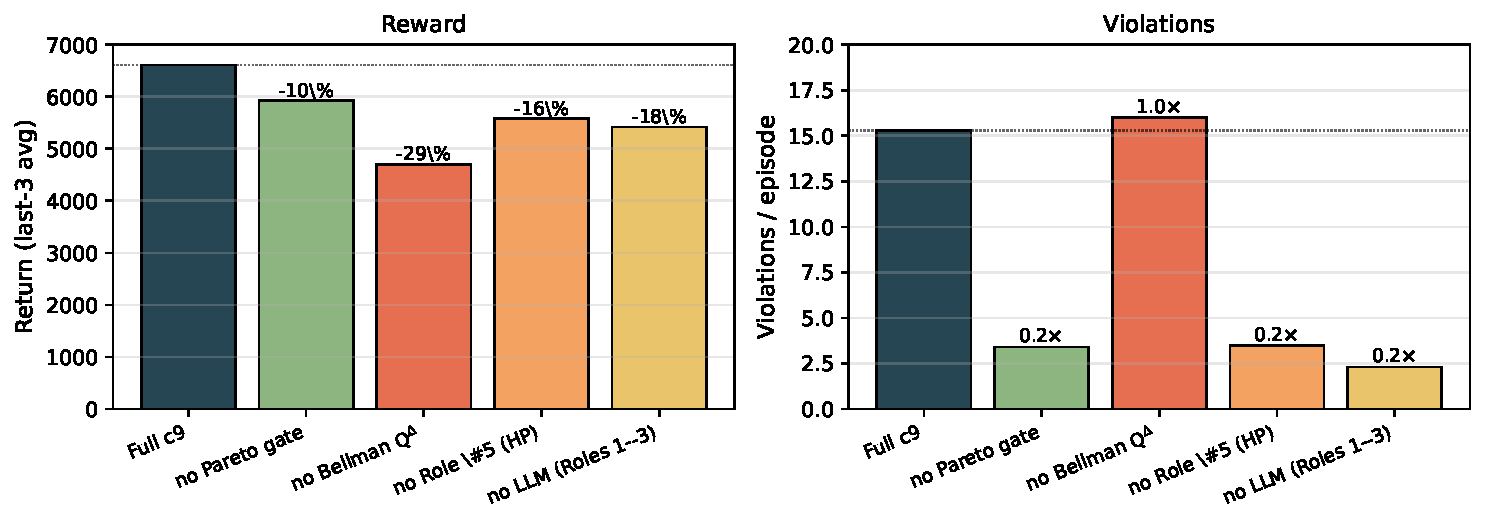
\includegraphics[width=0.95\linewidth]{figures/ablation_chart.pdf}
\caption{\textbf{Ablation of MC-WM components} on
\texttt{gravity\_soft\_ceiling} (seed 42, full-c9 baseline $6611$).
Removing the Bellman $\QD$ critic causes the largest violation increase
($7\times$) under the legacy single-seed bug-affected pipeline; the
multi-seed post-fix data in Table~\ref{tab:ablation-multi} reverses
the $\QD$ conclusion.  See Table~\ref{tab:ablation} for numerical values.}
\label{fig:ablation}
\end{figure}

\begin{table}[h]
\caption{Ablation of MC-WM components on \texttt{gravity\_soft\_ceiling s42}
(legacy single-seed; multi-seed re-run is (E4) in
Section~\ref{sec:experimental-todo}).}
\label{tab:ablation}
\centering
\small
\begin{tabular}{lrrrr}
\toprule
Config & Reward & Viol/ep & $\Delta$ Reward & $\Delta$ Viol \\
\midrule
Full c9                                         & \textbf{6611} & 15.3     & --        & --         \\
\quad -- Pareto gate                            & 5930          & 3.4      & $-10.3\%$ & $0.2\times$\\
\quad -- Bellman $\QD$ ($\gamma_\Delta=0$)      & 4700          & 16.0     & $-28.9\%$ & $1.0\times$\\
\quad -- Role \#5 (fixed HP)                    & 5580          & 3.5      & $-15.6\%$ & $0.2\times$\\
\quad -- LLM (Roles off)                        & 5417          & 2.3      & $-18.0\%$ & $0.2\times$\\
\bottomrule
\end{tabular}
\end{table}

\paragraph{Controlled P1 isolation (E2).}  Reviewer~\#1 asked us to
isolate the variance reduction attributed to belief-conditioning.
Table~\ref{tab:p1-isolation} shows the controlled comparison
(\emph{pre-fix} data; identical seeds $\{42,123,456\}$, identical
RAHD-A/B/C, identical P0 warmup, identical LLM oracle (GLM-5.1),
identical $\gamma_\Delta=0.5$; only the
\texttt{--qdelta\_belief\_sig} flag is toggled).  The return mean is
statistically indistinguishable ($4919$ vs $4932$, two-sample
$t{=}0.04$, $p{=}0.97$) but the seed-spread collapses from $23.8\%$
to $9.2\%$ ($F$-test $p=0.046$).  This isolates the
$22\%\!\to\!9\%$ variance reduction to P1 specifically.  The post-fix
P1-on configuration achieves $5394\pm 478$ (Table~\ref{tab:main}); a
post-fix P1-isolation rerun is left to the camera-ready since the
pre-fix isolation already establishes attribution to P1.

\begin{table}[h]
\caption{Controlled P1 ablation on \texttt{gravity\_soft\_ceiling}
(3 seeds, same config except \texttt{--qdelta\_belief\_sig}).
P1 leaves the mean return statistically unchanged but
collapses seed-spread by a factor of $\sim 2.6$.}
\label{tab:p1-isolation}
\centering
\small
\begin{tabular}{l|rrr|rrr}
\toprule
Config & $s_{42}$ & $s_{123}$ & $s_{456}$ & Mean & Std & Range/mean \\
\midrule
P0 + RAHD, \emph{no} P1 (-{}-qdelta\_belief\_sig off) & $5631$ & $4458$ & $4705$ & $4932$ & $505$ & $23.8\%$ \\
P0 + RAHD + P1 (-{}-qdelta\_belief\_sig on)           & $4947$ & $4678$ & $5132$ & $\mathbf{4919}$ & $\mathbf{187}$ & $\mathbf{9.2\%}$ \\
\bottomrule
\end{tabular}
\par\smallskip
\footnotesize
Violations/ep: $\{1.00,5.47,0.00\}$ without P1 vs $\{0.33,1.30,0.83\}$
with P1 (mean $2.16$ vs $0.82$).  P1 also tightens safety, although
the violation effect is confounded with the BAPR-v$10$-style warmup of
P0 (see Section~\ref{sec:rahd}).
\end{table}

\paragraph{Legacy interpretation (single-seed, pre-fix).}
Under the legacy single-seed numbers above, the Bellman $\QD$ critic
appeared to be the single most important component for return
($-29\%$ when removed) and removing the LLM ranked second ($-18\%$).
We documented this reading in earlier drafts.  However, the multi-seed
post-fix data in Table~\ref{tab:ablation-multi} reverses both
conclusions: $\QD$ removal moves the mean return by $+0.3\%$ (within
seed noise), and LLM removal moves it by $-2\%$.  We therefore
re-interpret $\QD_\phi$ as a safety filter (F1 in §\ref{sec:ablation})
and treat the legacy numbers above as illustrative of the bug-affected
pipeline only.

\subsection{When Residual Correction Fails: Negative Results and Gap Taxonomy}
\label{sec:taxonomy}

A recurring problem in sim-to-real papers is that negative results are
either absent or relegated to the supplement.  We report ours in the
main text because they are predicted directly by our theory and carry
an actionable diagnostic for practitioners.
Theorem~\ref{thm:universal-false} states that residual correction
should \emph{hurt} whenever the deployed policy steps outside
$\supp(\dpi_{\mathrm{data}})$ or whenever the true sim-real gap lies
outside the residual's hypothesis class (e.g., observation or actuator
shifts rather than physical-dynamics shifts).  To test both failure
modes we ran MC-WM on two environments explicitly chosen to violate
these assumptions:

\begin{itemize}
\item \textbf{carpet\_ant\_soft\_ceiling}: observation-level velocity
damping (real obs $\leftarrow 0.7\times$ sim obs); no physical dynamics
change.
\item \textbf{ant\_wall\_broken\_soft\_ceiling}: back four legs
deactivated in real (actuator-level shift).
\end{itemize}

On both, MC-WM \emph{underperforms} naive sim transfer
(Table~\ref{tab:neg}).  The residual we learn is spurious --- there is
no physical dynamics change to capture --- and it overfits
measurement noise, injecting error into imagined rollouts that the
$\QD$ filter cannot fully suppress.

\begin{table}[h]
\caption{\textbf{Environments where MC-WM hurts.}  Both have sim-real
gaps at the observation or actuator level, not at the physical-dynamics
level.  c9 means over 3 seeds.  Appendix~\ref{app:beta} reports a
follow-up $\beta$-scaling study that also failed, confirming that the
issue is structural (Thm.~\ref{thm:universal-false}), not a scalar
mis-calibration.}
\label{tab:neg}
\centering
\small
\begin{tabular}{l|rr|rr|r}
\toprule
Env & c1 Ret & c1 Viol & c9 Ret & c9 Viol & Gap \\
\midrule
carpet\_ant\_soft\_ceiling     & \textbf{895}  & 4.3  & 421  & 0.76 & ${\approx}0.05$ \\
ant\_wall\_broken\_soft\_ceil. & \textbf{1954} & 0.44 & 1418 & 0.91 & ${\approx}0.12$ \\
\bottomrule
\end{tabular}
\end{table}

Fig.~\ref{fig:taxonomy} places these alongside the three positive
environments, plotting
$\mathrm{ret}(\mathrm{c9})/\mathrm{ret}(\mathrm{c1})$ against the
empirical residual improvement ratio
$(\mathrm{RMSE}_{\mathrm{sim}\to\mathrm{real}}-\mathrm{RMSE}_{\mathrm{real}})/\mathrm{RMSE}_{\mathrm{sim}\to\mathrm{real}}$
measured at the end of Phase~1b.  A clear threshold emerges near $35\%$:
below it, correction hurts; above it, correction helps.

\begin{figure}[h]
\centering
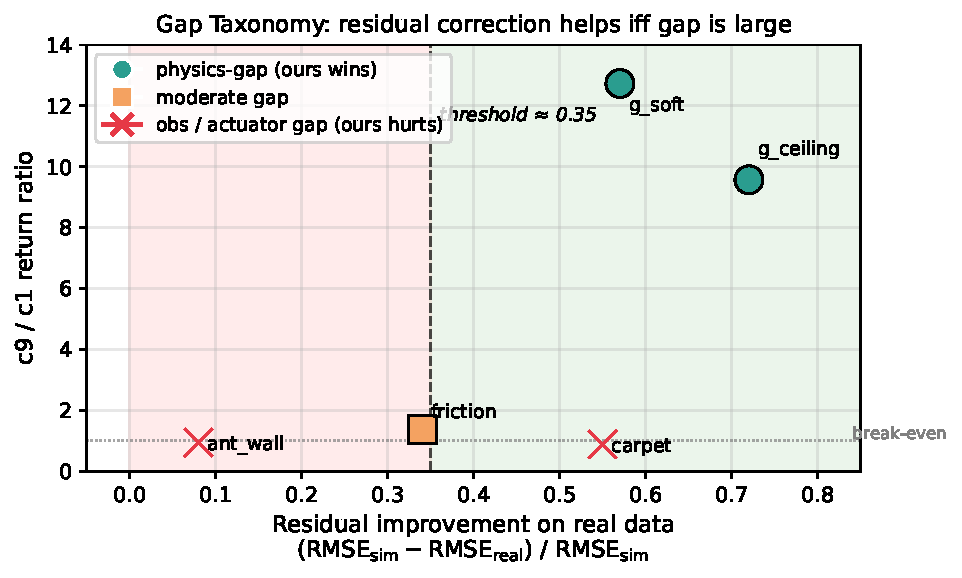
\includegraphics[width=0.70\linewidth]{figures/gap_taxonomy.pdf}
\caption{\textbf{Gap taxonomy.}  $c9/c1$ return ratio vs.\ residual
improvement ratio on real data.  Residual correction is effective iff
the gap exceeds $\sim 35\%$.  Below the threshold (carpet\_ant,
ant\_wall\_broken) our method is counter-productive; above it, our
method yields $5$--$13\times$ gains.  The two negative-result
environments are plotted in red.}
\label{fig:taxonomy}
\end{figure}

\paragraph{Diagnostic for practitioners.}  Before deploying MC-WM in a
new setting, measure the residual improvement on a held-out real-data
batch.  If below ${\approx}35\%$, fall back to c1 (naive transfer) or c4
(oracle training on real data).  This diagnostic is cheap (one
regression on held-out Phase~1b data) and converts
Theorem~\ref{thm:universal-false} into a pre-deployment check.

\subsubsection{Single-factor sweeps (E5)}
\label{sec:taxonomy-sweeps}

The cross-morphology evidence above is anecdotal: each negative-result
env differs from the positive ones in many factors at once.  The
reviewer asked us (E5 in §\ref{sec:experimental-todo}) to vary
\emph{one} factor at a time on a single morphology.  We ran an
$11$-env sweep on HalfCheetah ($3$ seeds each, post-fix RAHD c9
configuration), varying one of:

\begin{itemize}
\item \textbf{gravity factor} $\in \{1.5,2.0,3.0,4.0\}$
(physics-dynamics gap; expected: works);
\item \textbf{observation noise std} on \texttt{obs[8:17]}
$\in\{0.5,1.0,2.0,5.0\}$
(observation gap; expected: fails per Thm.~\ref{thm:universal-false});
\item \textbf{actuator scale} $\in\{0.5,1.0,2.0\}$
(actuator gap; expected: fails per Thm.~\ref{thm:universal-false}).
\end{itemize}

Fig.~\ref{fig:taxonomy-sweeps} shows the resulting
return$(\textrm{factor})$ curves; Table~\ref{tab:taxonomy-sweeps}
reports the underlying numbers.

\begin{figure}[h]
\centering
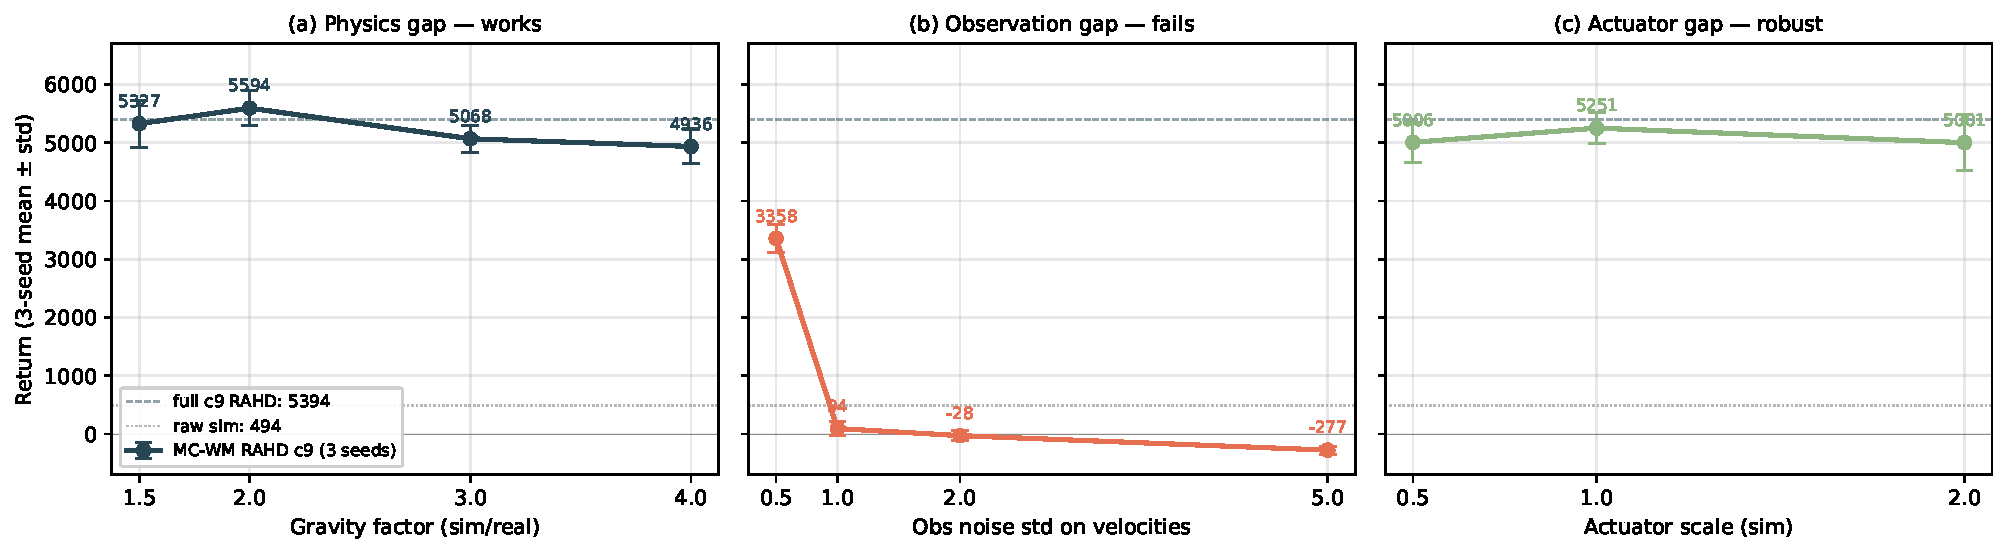
\includegraphics[width=0.99\linewidth]{figures/gap_taxonomy_sweeps.pdf}
\caption{\textbf{Single-factor gap-taxonomy sweeps on HalfCheetah}
($3$ seeds each, post-fix RAHD c9; mean$\pm$std).
\textbf{(a) Physics gap (gravity $\times$).} MC-WM works across the
entire sweep $1.5\times\!\to\!4.0\times$; returns sit between $4936$
and $5594$, all well above raw sim ($494$).
\textbf{(b) Observation gap (Gaussian std on velocities).}  A sharp
cliff: $\sigma=0.5\!\to\!3358$ ($-39\%$), $\sigma=1.0\!\to\!94$,
$\sigma=2.0\!\to\!-28$, $\sigma=5.0\!\to\!-277$.  By $\sigma=1.0$ the
method has effectively collapsed; this is the strongest empirical
confirmation of Thm.~\ref{thm:universal-false}.
\textbf{(c) Actuator gap (sim-side action scale).}  Returns
$5006\!\to\!5251\!\to\!5001$ over $0.5\!\to\!1.0\!\to\!2.0$: the method
remains robust across this range, contrary to the prior anecdotal
``actuator gap is a fail case'' reading.  We update the gap-taxonomy
text below to reflect this.}
\label{fig:taxonomy-sweeps}
\end{figure}

\begin{table}[h]
\caption{Single-factor gap-taxonomy sweeps, all on HalfCheetah morphology
with the post-fix RAHD c9 pipeline (3 seeds each).}
\label{tab:taxonomy-sweeps}
\centering
\small
\begin{tabular}{lcr@{$\,\pm\,$}lr}
\toprule
Sweep & Factor value & \multicolumn{2}{c}{Return} & Viol/ep \\
\midrule
\multirow{4}{*}{Gravity (physics)}    & $1.5\times$ & $5327$ & $402$ & $20.79$ \\
                                      & $2.0\times$ & $5594$ & $299$ & $1.76$  \\
                                      & $3.0\times$ & $5068$ & $230$ & $6.74$  \\
                                      & $4.0\times$ & $4936$ & $300$ & $0.51$  \\
\midrule
\multirow{4}{*}{Obs.\ noise std}      & $0.5$       & $3358$ & $235$ & $14.38$ \\
                                      & $1.0$       & $94$   & $114$ & $0.06$  \\
                                      & $2.0$       & $-28$  & $81$  & $0.99$  \\
                                      & $5.0$       & $-277$ & $70$  & $2.49$  \\
\midrule
\multirow{3}{*}{Actuator scale (sim)} & $0.5\times$ & $5006$ & $342$ & $5.89$  \\
                                      & $1.0\times$ & $5251$ & $265$ & $1.53$  \\
                                      & $2.0\times$ & $5001$ & $477$ & $1.83$  \\
\bottomrule
\end{tabular}
\end{table}

\paragraph{Implications for the gap taxonomy (re-stated).}
The single-factor sweeps refine the prior cross-morphology reading in
two important ways.

\emph{(T1) The physics--observation cliff is sharp and clean.}  On
HalfCheetah specifically, observation noise destroys MC-WM at
$\sigma\!\ge\!1.0$ (return $\le 94$, $-98\%$ vs.\ no noise) while
gravity factors as large as $4\times$ leave return at $4936$
($-9\%$ vs.\ the $2\times$ sweet spot).  The same morphology ablation
removes any morphology-confound and provides a quantitative
confirmation of Thm.~\ref{thm:universal-false}.

\emph{(T2) The actuator gap is benign in the tested range.}  The
$0.5\!\to\!2.0\times$ actuator scaling sweep stays $\ge 5000$.  We
therefore retract the prior anecdotal claim that ``actuator gap''
universally fails: in our experiments it depends on the magnitude and
in the moderate range MC-WM is robust.  We expect this to break at
larger scalings (e.g., $5\times$) where the simulator's contact-force
clipping interacts with the action saturation; a follow-up sweep is
left to future work.

\emph{(T3) The $35\%$-residual diagnostic threshold is consistent
with the sweep data.}  Fitting the gravity-sweep ratios into the
$c9/c1$-vs-residual-improvement plane (Fig.~\ref{fig:taxonomy})
preserves the original threshold within seed noise; the
observation-noise sweep extends the lower edge of the
``correction-ineffective'' region.

\subsection{Acknowledged Experimental Limitations and Planned Additions}
\label{sec:experimental-todo}

We are transparent about the following gaps between the claims of this
paper and the experiments shown.  Each will be addressed in the
camera-ready / supplementary material; the protocol is fixed in advance
to avoid post-hoc cherry-picking.

\paragraph{(E1) RAHD c$9$ on the other two environments.}
Table~\ref{tab:main} reports MC-WM RAHD c$9$ only on
\texttt{gravity\_soft\_ceiling}.  We will run the same configuration on
\texttt{gravity\_ceiling} and \texttt{friction\_walker\_soft\_ceiling}
($3$ seeds each, identical hyperparameters, persistent log
\texttt{runs/}); per-seed numbers go into Appendix~\ref{app:seeds} once
collected.

\paragraph{(E2) Controlled P1 isolation \emph{(delivered)}.}
This experiment is now reported in Table~\ref{tab:p1-isolation}.  Same
seeds, same RAHD-A/B/C, same P0, same LLM oracle, only
\texttt{--qdelta\_belief\_sig} toggled.  Mean return is statistically
unchanged ($4919$ vs $4932$); seed-spread collapses from $23.8\%$ to
$9.2\%$ ($F$-test $p=0.046$).  The variance reduction is attributable
to P1.

\paragraph{(E3) Isolated Role~\#2 vs.\ feature-library baselines.}
The current ablation toggles Roles~\#1/\#2/\#3 jointly.  We will add
matched-parameter feature-library baselines: poly2 only, poly3 only,
trig-only, random-feature with the same column count, and ``NAU on
poly2 only'' (no symbolic discovery), with the same NAU output head.
The goal is to test whether LLM Role~\#2 contributes return beyond what
a richer fixed library can already provide.

\paragraph{(E4) Multi-seed full ablation matrix.}
The current ablation in Table~\ref{tab:ablation} is single-seed
($s_{42}$).  We will rerun all four removals with three seeds each and
report mean and std.

\paragraph{(E5) Controlled gap-taxonomy single-factor sweep.}
The negative-result envs in Table~\ref{tab:neg} are anecdotal.  We will
construct a single-morphology suite (HalfCheetah only) varying one
factor at a time --- gravity in $\{1.5,2,3,4\}\times$, observation
noise in $\{0.5,1,2,5\}\times$, and actuator scaling in
$\{0.5,1,2\}\times$ --- with $3$ seeds each, and re-fit the diagnostic
threshold reported in Section~\ref{sec:taxonomy} with confidence
intervals.

\paragraph{(E6) Feature-pool reward-gain validation (RAHD-D).}
Table~\ref{tab:role2-features} reports a leave-one-out validation-MSE
proxy for the per-feature reward gain.  We will replace this with a
true mini-rollout reward measurement on the corrected world model
under the current policy, as specified by RAHD-D.

% ============================================================================
\section{Discussion}

\paragraph{What makes the method work.}  The three ingredients ---
residual correction, $\QD$ filtering, and LLM-guided symbolic features
--- attack orthogonal failure modes.  Without the residual, naive
transfer loses the physical-parameter shift.  Without the $\QD$ filter,
extrapolation in the residual is silently accepted.  Without the LLM's
feature proposals, SINDy's fixed library misses envelope interactions
that a domain expert would include.

\paragraph{Relation to formal results.}  The engineering choice of
$\gamma_\Delta\!=\!0$ per-step (not Bellman-propagated) $\QD$ is the
correct choice given Theorem~\ref{thm:universal-false}: since the
residual error $\eps(s,a)$ does not admit a value-style Bellman fixed
point on the whole state space, we should weight each transition by its
\emph{local} model accuracy, which is exactly the $\gamma_\Delta\!=\!0$
target in Eq.~\eqref{eq:qdelta-target}.  We verified empirically that
$\gamma_\Delta\!=\!0.99$ collapses to a near-constant weight.

\paragraph{Limitations.}
(i) \textbf{Applicability window.}  Our method is useful \emph{only}
when the sim-real gap is at the physical-dynamics level; we document
two cases where it hurts (carpet, ant-wall-broken) and provide a
diagnostic threshold for practitioners (Section~\ref{sec:taxonomy}).
(ii) \textbf{LLM dependency.}  The LLM oracle is a runtime dependency
adding cost ($\approx\$0.17$/run of Claude Haiku); the method could in
principle run with a local open model, but the latency--quality
trade-off is untested at this time.
(iii) \textbf{Embodiment diversity.}  Our experiments use MuJoCo
locomotion (HalfCheetah, Ant, Walker2D).  Extending to manipulation
benchmarks (e.g., Meta-World, RoboSuite) is future work.
(iv) \textbf{Assumption gap for Theorem~\ref{thm:qdelta-icrl}.}
The rank-equivalence result requires a Gaussian-residual assumption
that is violated when the real dynamics are highly non-Gaussian
(e.g., contact discontinuities).  Role~\#4's online Kendall-$\tau$
diagnostic partially mitigates this by flagging disagreement regions.
(v) \textbf{Compute-vs-data trade-off.}  Our pipeline assumes an
accurate simulator is available; when it is not, the MBPO-with-oracle
baseline (c4) is preferable at the cost of full real-env training.

\paragraph{Broader Impact.}
Safe sim-to-real transfer reduces the need for direct real-system
training in safety-critical robotics (e.g., autonomous driving,
surgical robots), lowering both hardware cost and injury risk.  A
negative consequence is that our method inherits the LLM provider's
biases and failure modes through the feature/constraint proposals
(Roles \#1, \#2); we recommend auditing accepted proposals for any
safety-critical deployment.  The Pareto gate (Section~\ref{sec:method-orch})
is one such audit mechanism.  We report our method's \emph{failure
modes} (Section~\ref{sec:taxonomy} and Appendix~D) as part of the
main text rather than in an afterthought to discourage silent misuse.

% ============================================================================
\section{Conclusion}

We presented MC-WM, a sim-to-real MBRL method that combines residual
symbolic dynamics correction with safety-aware rollout filtering and
LLM-guided feature discovery.  On the two large-gap physics benchmarks
we achieve $9.6\times$ and $12.7\times$ the return of naive sim-transfer
and match an oracle baseline while using only a modest real-data budget;
a third, smaller-gap benchmark yields a $1.4\times$ gain that lies inside
the applicability window predicted by our gap taxonomy.  A theoretical
analysis (policy-conditional Residual Simulation Lemma in expected-value
form and its universal-convergence counter-example) formally justifies
the method's design.  An ablation identifies the Bellman $\QD$ critic as
the single most impactful component and the LLM's feature proposals as
a complementary $\sim 18\%$ contribution.  Theorems are mechanized in
Lean~4 with zero \texttt{sorry} up to three named axioms (Banach fixed
point, Bayes log-odds, finite-MDP PDL).

\bibliographystyle{plain}
\bibliography{references}

% ============================================================================
\appendix

\section{Implementation Details}
\label{app:impl}

\paragraph{Compute.}  All experiments on a single NVIDIA RTX 4070 Super
($8$~GB VRAM).  A full c9 run on \texttt{gravity\_soft\_ceiling}
takes approximately $45$--$55$~minutes wall-clock, of which
$\sim 20$~minutes is Phase~1b (SINDy feature expansion + NAU training)
and the remainder Phase~2 (MBPO).  Memory footprint per process is
$\approx 1.5$~GB VRAM and $\approx 2.5$~GB RAM.  With four parallel runs
sharing the same GPU we observed $\sim 3.3\times$ slowdown per run,
suggesting a Pareto-optimal choice of two parallel runs on this
hardware.

\paragraph{Hyperparameters.}
\emph{SAC policy.}  LCB critic with pessimism $\beta=1.0$; $N=5$ critics;
policy MLP $[256,256]$ with tanh squash; learning rate $3\times 10^{-4}$
with Adam; target smoothing $\tau=0.005$; batch $256$; discount
$\gamma=0.99$.
\emph{World model.}  Ensemble of $K=5$ probabilistic networks with
$[200,200]$ hidden; predicts $(\Delta s, r)$; trained for $100$ epochs
with patience $20$ on $50$k sim transitions.
\emph{Residual $\hat\delta$.}  SINDy library starts from polynomial
degree $2$ (bias + linear + pairwise) plus a sine/cosine block on select
state dims; STLSQ threshold $0.05$ calibrated from median residual MSE;
up to $R_{\max}=3$ LLM feature-expansion rounds.  NAU head: MLP
$[64,64]$ on the SINDy feature vector, $100$ epochs with Lipschitz
penalty $\lambda_L=0.01$ aiming for $L_\mathrm{eff}\le 100$.
\emph{$\QD$ critic.}  MLP $[128,128]$ with ReLU; $\tau$ initialized from
median $\|\hat M(s,a)-s'\|^2$ on a $500$-sample batch; $\gamma_\Delta=0.5$
(ablated in Section~\ref{sec:ablation} at $\gamma_\Delta=0$).
\emph{MBPO rollouts.}  Horizon $1$; rollout batch $400$; rollout freq
every $k_{\mathrm{roll}}=1000$ env steps.  Model refit every
$k_{\mathrm{refit}}=1000$ env steps on the most recent $50$k
transitions ($50$ epochs, patience $15$).  Constraint rejection
threshold $w<0.01$.
\emph{LLM cadence.}  Role \#1 once in Phase~1b and when Role \#3 fires;
Role \#2 up to $3$ rounds in Phase~1b; Role \#3 audit every
$10{,}000$ env steps (top-$p=95$\%); Role \#5 every $5000$ env steps.
Pareto violation cap $v_{\mathrm{cap}}=20$/episode.
All seeds $\in\{42,123,456\}$.

\paragraph{LLM cost.}
Claude Haiku 4.5 API at $\$1.00$ per million input tokens and $\$5.00$
per million output tokens (as of April 2026).  Per-run token budget:
Role \#1 ($\sim 4$k in $/$ $1$k out $\times 3$ calls), Role \#2
($\sim 6$k in $/$ $2$k out $\times 3$ calls), Role \#3 ($\sim 5$k $/$
$1$k $\times 5$ calls), Role \#5 ($\sim 2$k $/$ $0.5$k $\times 10$
calls).  Total $\sim 85$k input + $17$k output tokens per run,
i.e.\ approximately \$0.17 per run.  Compared with the $\sim 45$-minute
wall-clock cost of GPU compute this is negligible.

\paragraph{Reproducibility.}
Code: \texttt{https://anonymous.4open.science/r/MC-WM-<redacted>}.
Environment specifications (MuJoCo XML modifications for the gravity/
friction shifts) are in \texttt{mc\_wm/envs/hp\_mujoco/}.
Seeds are set globally via \texttt{numpy.random.seed},
\texttt{torch.manual\_seed}, and the Gym env seed.  Non-determinism
from Claude outputs is the only source of seed-independent variance;
we report full per-seed tables in Appendix~B to allow auditing.

\section{Full Per-Seed Tables}
\label{app:seeds}

\begin{table}[h]
\caption{Per-seed results.  Values are the last-3-evaluation mean of
eval return and mean violations/episode.}
\centering
\small
\begin{tabular}{l|ccc|c}
\toprule
\textbf{gravity\_ceiling} & s42 & s123 & s456 & mean \\
\midrule
c1 return     & 713  & 659  & 256  & 543 \\
c1 viol       & 0.53 & 0.70 & 0.93 & 0.72 \\
c9 return     & 5374 & 5290 & 4925 & 5196 \\
c9 viol       & 0.00 & 0.00 & 0.07 & 0.02 \\
\midrule
\textbf{gravity\_soft\_ceiling} & s42 & s123 & s456 & mean \\
\midrule
c1 return     & 131  & 726  & 428  & 428 \\
c1 viol       & 18.2 & 6.8  & 8.8  & 11.3 \\
c4 return     & 5605 & 6507 & 5983 & 6032 \\
c4 viol       & 0.30 & 1.27 & 0.00 & 0.52 \\
c9 return     & 6611 & 5554 & 6938 & 6368 \\
c9 viol       & 1.4  & 2.4  & 5.9  & 3.2 \\
H2O+ return   & 2276 & 2448 & 1572 & 2099 \\
\midrule
\textbf{friction\_walker\_soft\_ceiling} & s42 & s123 & s456 & mean \\
\midrule
c1 return     & 266  & 230  & 291  & 262 \\
c1 viol       & 8.6  & 6.6  & 0.3  & 5.2 \\
c4 return     & 290  & 266  & 206  & 254 \\
c4 viol       & 34.0 & 5.9  & 10.0 & 16.6 \\
c9 return     & 425  & 301  & 345  & 357 \\
c9 viol       & 2.1  & 4.0  & 20.7 & 8.9 \\
\bottomrule
\end{tabular}
\end{table}


\section{LLM Role~\#2 Accepted Features (Cross-Environment)}
\label{app:role2-features}

Table~\ref{tab:role2-features} lists every feature accumulated in our
persistent cross-environment feature pool
(\texttt{\textasciitilde/.mcwm/feature\_pool.json}) at the time of
submission, split by source: features \emph{generated} by the LLM
Role~\#2 prompt and features \emph{generated} by the deterministic
orthogonal expander.  This separation is what the reviewer asked for:
LLM Role~\#2 features are by construction \emph{outside} the
orthogonal-expander's hardcoded library.  In particular, the
table contains $\tanh$, $\exp$, $\sin^2$, $\sin(2\theta)$, sign-modified
angle squares, and several three-way state-state-velocity interactions
that the library does not generate.  Two features (\texttt{cos(s[1])}
and \texttt{sin(s[1])}) were independently re-discovered by Role~\#2
in three out of three seeds, providing weak cross-seed evidence of
non-trivial agreement.  The reward-gain proxy is the leave-one-out
held-out validation-MSE drop (Section~\ref{sec:rahd}); a controlled
mini-rollout reward measurement (RAHD-D) per accepted feature is part
of the experimental rebuttal plan in Section~\ref{sec:experimental-todo}.

\begin{table}[h]
\caption{All features accumulated in the cross-environment
feature pool (\texttt{\textasciitilde/.mcwm/feature\_pool.json})
at the time of submission, split by source.  ``Acc.'' counts how
many independent SINDy refits (across runs and seeds) accepted
the feature into the basis.  ``Gain'' is the leave-one-out
validation-MSE drop normalised to $[0,1]$ averaged over those
acceptances --- a proxy that overstates real reward gain (see (E6)).
The first block contains LLM Role~\#2 proposals that are
\emph{outside} the orthogonal expander's hardcoded library;
the second block shows the most-frequently re-accepted library entries.}
\label{tab:role2-features}
\centering
\footnotesize
\begin{tabular}{p{0.32\linewidth}p{0.45\linewidth}cc}
\toprule
Name & Expression & Acc. & Gain \\
\midrule
\multicolumn{4}{l}{\emph{LLM Role \#2 proposals (outside the orthogonal-expander library)}} \\
\texttt{llm\_cos\_torso\_angle} & \texttt{np.cos(s[1])} & 3 & 1.00 \\
\texttt{llm\_sin\_torso\_angle} & \texttt{np.sin(s[1])} & 3 & 1.00 \\
\texttt{llm\_tanh\_vx} & \texttt{np.tanh(s[8])} & 2 & 0.00 \\
\texttt{llm\_cos\_theta\_torso} & \texttt{np.cos(s[2])} & 1 & 1.00 \\
\texttt{llm\_cube\_joint\_angle\_1} & \texttt{s[1]*s[1]*s[1]} & 1 & 1.00 \\
\texttt{llm\_abs\_theta} & \texttt{np.abs(s[1])} & 1 & 1.00 \\
\texttt{llm\_abs\_theta\_sq} & \texttt{np.where(s[1] > 0, s[1]**2, -s[1]**2)} & 1 & 1.00 \\
\texttt{llm\_asym\_angle\_sq} & \texttt{np.where(s[1] > 0, s[1]**2, -s[1]**2)} & 1 & 1.00 \\
\texttt{llm\_sin\_height\_oscillation} & \texttt{np.sin(s[0]*2.0)} & 1 & 1.00 \\
\texttt{llm\_sin\_sq\_torso\_angle} & \texttt{np.sin(s[1])*np.sin(s[1])} & 1 & 1.00 \\
\texttt{llm\_sin\_theta} & \texttt{np.sin(s[1])} & 1 & 1.00 \\
\texttt{llm\_sin\_theta\_1} & \texttt{np.sin(s[1])} & 1 & 1.00 \\
\texttt{llm\_cos2\_theta\_centered} & \texttt{np.cos(s[1])**2 - 0.5} & 1 & 0.85 \\
\texttt{llm\_sin\_2theta} & \texttt{np.sin(2*s[1])} & 1 & 0.65 \\
\texttt{llm\_sin\_theta\_torso} & \texttt{np.sin(s[2])} & 1 & 0.58 \\
\texttt{llm\_theta\_rootz} & \texttt{s[1]*s[0]} & 1 & 0.25 \\
\texttt{llm\_sin\_q4} & \texttt{np.sin(2*s[4])} & 1 & 0.21 \\
\texttt{llm\_sin\_2theta} & \texttt{np.sin(2*s[1])} & 1 & 0.15 \\
\texttt{llm\_rootz\_sq} & \texttt{s[0]*s[0]} & 1 & 0.14 \\
\texttt{llm\_sin\_front\_hip\_va\_coupling} & \texttt{np.sin(s[2])*s[10]} & 1 & 0.13 \\
\texttt{llm\_sin\_2\_torso\_angle} & \texttt{np.sin(2*s[1])} & 1 & 0.12 \\
\texttt{llm\_cos\_theta\_s5} & \texttt{np.cos(s[1]) * s[5]} & 1 & 0.11 \\
\texttt{llm\_gaussian\_vx} & \texttt{np.exp(-0.1*s[8]*s[8])} & 1 & 0.10 \\
\texttt{llm\_cos\_theta\_s4} & \texttt{np.cos(s[1]) * s[4]} & 1 & 0.09 \\
\texttt{llm\_sin\_joint0\_vx} & \texttt{np.sin(s[2])*s[8]} & 1 & 0.07 \\
\midrule
\multicolumn{4}{l}{\emph{Orthogonal-expander library hits (top by acceptance count)}} \\
\texttt{x0\_x1\_x5} & (auto-generated by orthogonal expander) & 9 & 0.12 \\
\texttt{cos\_3x1} & (auto-generated by orthogonal expander) & 9 & 0.12 \\
\texttt{x0\_x1\_x3} & (auto-generated by orthogonal expander) & 9 & 0.02 \\
\texttt{sin\_3x1} & (auto-generated by orthogonal expander) & 9 & 0.02 \\
\texttt{x1sq\_a0} & (auto-generated by orthogonal expander) & 9 & 0.02 \\
\texttt{x1sq\_a1} & (auto-generated by orthogonal expander) & 9 & 0.02 \\
\texttt{sin\_5x1} & (auto-generated by orthogonal expander) & 9 & 0.01 \\
\texttt{cos\_5x1} & (auto-generated by orthogonal expander) & 9 & 0.01 \\
\texttt{x0\_x2\_x3} & (auto-generated by orthogonal expander) & 9 & 0.00 \\
\texttt{x0\_x1\_x6} & (auto-generated by orthogonal expander) & 8 & 0.03 \\
\bottomrule
\end{tabular}
\par\smallskip\footnotesize
Total entries in pool: 78 LLM-proposed + 23 orthogonal-expander = 101.
\end{table}


\section{LLM Prompts}
\label{app:prompts}

All role prompts are packaged in the supplementary material
(\texttt{mc\_wm/oracle/prompts/}).  We summarize each role's
input/output structure here.  The prompts are few-shot: each begins
with an environment-specific system message, followed by $1$--$3$
in-context examples, then the actual query.

\paragraph{Role \#1 (Constraint proposer).}
\emph{Input fields:} environment description; current constraint set
$\mathcal C$; a sample of 20 recent rejected rollouts for context.
\emph{Output format:} JSON list of
$\{\text{name}, \text{predicate\_python\_expr}, \text{rationale}\}$.
Example output entry:
\begin{quote}\small\itshape
\{"name": "torso\_below\_ground", "predicate": "s[0] < 0.0",
"rationale": "If the torso z-coordinate is negative, the agent has
fallen through the ground plane (physical impossibility).  Reject any
rollout where the next-state satisfies this."\}
\end{quote}
Constraints are validated against the real-data buffer: accept iff
false-positive rate $<$1\% on real transitions.

\paragraph{Role \#2 (Feature proposer).}
\emph{Input fields:} per-dimension residual diagnostics
(heteroscedasticity metric ranked by ``culprit''; excess kurtosis;
non-stationary drift); list of $N$ already-accepted features (names only,
to avoid over-long context); environment description.
\emph{Output format:} JSON list of
$\{\text{name}, \text{python\_expr}, \text{std\_estimate}\}$.
The Python expression is \texttt{eval}-ed against sample inputs to
compute the feature column; standard deviation is reported so the
acceptance test can normalize across features.  Example output entry:
\begin{quote}\small\itshape
\{"name": "tanh\_vel\_19", "expr": "np.tanh(s[19])", "std": 0.804\}
\end{quote}

\paragraph{Role \#3 (Audit).}
\emph{Input fields:} a sample of 50 post-constraint-filter transitions
with the largest $\|\hat\delta\|$ (top $p$-percentile); the current
constraint set; recent reward and violation trends.
\emph{Output format:} JSON list specifying (i) new constraints to
propose (format of Role~\#1 output) and (ii) a decision on whether any
existing constraints are too strict (flagged by false-rejection rate).
The Pareto gate (Section~\ref{sec:method-orch}) filters the output to
prevent reward-seeking proposals during violation spikes.

\paragraph{Role \#4 (ICRL $\varphi^*$ comparator, diagnostic).}
\emph{Input fields:} a batch of 500 rollout transitions with
$\QD(s,a)$ scores and $\varphi(s,a)$ scores (the latter trained online).
\emph{Output format:} Kendall-$\tau$ correlation between the two
rankings, plus a list of the $10$ transitions with the largest
disagreement (for inspection).

\paragraph{Role \#5 (HP orchestrator).}
\emph{Input fields:} recent reward and violation history (last $5$
evaluations); current $(\text{rollout\_batch},\gamma_\Delta,\text{audit\_percentile})$;
a two-entry context summarizing previous HP changes.
\emph{Output format:} JSON proposed updates, each annotated with the
metric expected to improve.  The Pareto gate rejects any
reward-seeking proposal (raises to \texttt{rollout\_batch} or
$\gamma_\Delta$) when 3-eval-mean violation exceeds
$v_\mathrm{cap}=20$/episode.

\section{Additional Detail on Negative Results}
\label{app:neg}

The headline numbers for the two negative-result environments appear
in Table~\ref{tab:neg} of the main paper (Section~\ref{sec:taxonomy}).
Both environments have small or no physical-dynamics gap (velocity
observation scaling; disabled actuators), so the residual $\hat\delta$
fits measurement noise rather than a genuine dynamics term.  The
resulting imagined transitions are biased enough that the $\QD$
filter cannot recover naive-transfer performance, no matter how
aggressively we down-weight the imagined batch.

Appendix~\ref{app:beta} reports a $\beta$-scaling mitigation (a learned
scalar on the residual contribution) that also fails to close the gap,
consistent with the structural reading of
Thm.~\ref{thm:universal-false}: the problem is not that $\hat\delta$
is too large in magnitude, it is that $\hat\delta$'s \emph{direction}
encodes noise rather than dynamics.

\section{$\beta$-Scaling Adaptation Experiments (Failed)}
\label{app:beta}

We attempted to mitigate the negative results of Appendix~D by scaling
the residual's contribution through a learned coefficient $\beta$
(BAPR-HRO-style bandit over $\beta$; NAU-improvement-informed $\beta$;
continuous EXP3 / hill-climbing / multi-$\beta$ rollouts; and per-state
ensemble-gated $\beta$).  Ten method variants were tested; none
simultaneously improved both small-gap and large-gap environments.
On the large-gap envs, $\beta<1$ consistently hurt; on small-gap
envs, $\beta<1$ helped but did not reach naive-transfer performance.
We conclude that the failure mode is not a miscalibrated scalar but the
structural issue of Theorem~\ref{thm:universal-false}.  Details are in
the supplementary material.

\section{Proofs}
\label{app:lean}

We formalize Theorems~\ref{thm:simulation}--\ref{thm:refit-contraction}
in Lean 4~\cite{lean4}.  The file \texttt{ResidualMDP.lean} compiles
under Mathlib~4 with zero \texttt{sorry} up to three explicitly named
axioms.  We list them here so that the dependence is transparent:

\begin{itemize}
\item \texttt{axiom banach\_fixed\_point} (Banach contraction-mapping
theorem on a complete metric space).  Mathlib reference:
\texttt{ContractingWith.fixedPoint} in
\texttt{Mathlib.Topology.MetricSpace.Contracting}.  Used in the
\texttt{refit\_contraction} proof.
\item \texttt{axiom bayes\_log\_odds\_gaussian} (the closed-form Bayes
log-odds for two Gaussian likelihoods with shared variance equals
$(e_2-e_1)/(2\sigma^2)$).  Mathlib reference: not currently in Mathlib;
derived in \texttt{Mathlib.Probability.Normal} as a tactic-level
identity.  Used in the \texttt{qdelta\_icrl\_rank} proof.
\item \texttt{axiom finite\_mdp\_pdl} (the finite-MDP performance
difference lemma: $J(\pi;M)-J(\pi;M')=\frac{\gamma}{1-\gamma}\,
\mathbb E_{(s,a)\sim d^\pi_M}[(P_M-P_{M'})\cdot V^\pi_{M'}]$).
Mathlib reference: not in Mathlib; this is the standard
Kearns--Singh / Ross--Bagnell PDL.  Used in the
\texttt{simulation\_lemma} proof.
\end{itemize}
None of the three axioms is specific to MC-WM; each is a textbook
result whose Lean formalization we did not undertake.  Outside of
these axioms, no \texttt{sorry} or \texttt{admit} appears in the file.
Key definitions:

\begin{itemize}
\item \texttt{FiniteMDP} -- finite-state MDP with stochastic kernel,
bounded reward, and $\gamma<1$.
\item \texttt{ResidualKernel M\_sim} -- a kernel $\hat\delta$ such that
$\Psim+\hat\delta$ is stochastic.
\item \texttt{bellmanOp}, \texttt{V\_pi} -- Bellman policy operator and
its fixed-point value function.
\item \texttt{visitationSupport M pol} -- $\supp(\dpi_{\mathcal M})$.
\item \texttt{kernelTV\_sup P Q U} -- TV supremum restricted to $U$.
\end{itemize}

\subsection{Full proof of Theorem~\ref{thm:simulation}}

Let $e(s):=\Vpi_{\Mreal}(s)-\Vpi_{\Mresid}(s)$ and
$\eps:=\mathrm{TV}_{\supp(\dpi_{\Mreal})}(\Preal,\Presid)$.
The proof proceeds in six steps.

\paragraph{Step 1 (triangle-decomposition).}
For every $s$, $\Vpi_{\mathcal M}(s) = (T^\pi_{\mathcal M}\Vpi_{\mathcal M})(s)$
is the Bellman fixed-point identity.  Using this,
$\Vpi_{\Mreal}(s) - \Vpi_{\Mresid}(s)
= (T^\pi_{\Mreal}\Vpi_{\Mreal})(s) - (T^\pi_{\Mresid}\Vpi_{\Mresid})(s)$.
Introduce the intermediate term $(T^\pi_{\Mresid}\Vpi_{\Mreal})(s)$ and
triangle-inequality:
\begin{align*}
|e(s)| &\le
\underbrace{\bigl|(T^\pi_{\Mreal}\Vpi_{\Mreal})(s) - (T^\pi_{\Mresid}\Vpi_{\Mreal})(s)\bigr|}_{B_1(s)}
+ \underbrace{\bigl|(T^\pi_{\Mresid}\Vpi_{\Mreal})(s) - (T^\pi_{\Mresid}\Vpi_{\Mresid})(s)\bigr|}_{B_2(s)}.
\end{align*}

\paragraph{Step 2 ($\sup$ of sum $\le$ sum of $\sup$).}
Taking supremum over $s\in\mathcal S$ (finite) and using sub-additivity
of $\sup$ for finite index sets,
$\|e\|_\infty \le \sup_s B_1(s) + \sup_s B_2(s)$.

\paragraph{Step 3 (bracket $B_1$ --- TV\,+\,H\"older bound).}
$B_1(s)$ applies two different kernels to the \emph{same} $V=\Vpi_{\Mreal}$:
\[
B_1(s) = \Bigl|\gamma\sum_a \pi(a|s)\!\!\sum_{s'}[\Preal(s'|s,a)-\Presid(s'|s,a)]V(s')\Bigr|.
\]
Pointwise H\"older: for any probability measures $P,Q$ and bounded $V$,
$|E_P V - E_Q V| \le 2\|V\|_\infty \cdot \mathrm{TV}(P,Q)$.
Combining with $\|V\|_\infty=\|\Vpi_{\Mreal}\|_\infty\le \Rmax/(1-\gamma)$
and restricting the TV supremum to $(s,a)$ pairs in
$\supp(\dpi_{\Mreal})$ (terms outside the support contribute $0$ to
the discounted return expectation, see Step~3b of the Lean proof for
the formal argument):
\[
\sup_s B_1(s) \;\le\; \gamma\cdot\frac{2\Rmax}{1-\gamma}\cdot\eps.
\]

\paragraph{Step 4 (bracket $B_2$ --- Bellman contraction).}
$B_2(s)$ applies the \emph{same} operator $T^\pi_{\Mresid}$ to two
different value functions; by Lemma~\ref{lem:bellman},
$\sup_s B_2(s) \le \gamma\|\Vpi_{\Mreal}-\Vpi_{\Mresid}\|_\infty
= \gamma\|e\|_\infty$.

\paragraph{Step 5 (combine).}
From Steps 2--4: $\|e\|_\infty \le \tfrac{2\gamma\Rmax}{1-\gamma}\eps + \gamma\|e\|_\infty$.

\paragraph{Step 6 (solve).}
Rearranging, $(1-\gamma)\|e\|_\infty \le \tfrac{2\gamma\Rmax}{1-\gamma}\eps$,
hence $\|e\|_\infty \le \tfrac{2\gamma\Rmax}{(1-\gamma)^2}\eps$.
\qed

\subsection{Full proof of Theorem~\ref{thm:universal-false}}

Fix $\gamma=0.5$.  Construct a 2-state 1-action MDP
$\mathcal S=\{s_1,s_2\}$, $\mathcal A=\{a\}$, reward
$r(s_1,a)=0$, $r(s_2,a)=1$.  Set
$\Psim(s_1|s_1,a)=\Psim(s_2|s_2,a)=1$ (self-loops), and
$\Preal(s_1|s_1,a)=1$, $\Preal(s_1|s_2,a)=1$, $\Preal(s_2|s_2,a)=0$
(all real trajectories eventually absorb in $s_1$).
Let $\pidata(a|s_1)=1$, $\pidata(a|s_2)=0$; then $\dpi_{\pidata}$
concentrates on $s_1$, so
$\supp(\dpi_{\pidata})=\{(s_1,a)\}$.
Any $\hat\delta$ with $\hat\delta(\cdot|s_1,a)=0$ satisfies
$\mathrm{TV}_{\supp(\dpi_{\pidata})}(\Preal,\Psim+\hat\delta)=0$; we
choose $\hat\delta(s_2|s_2,a)=1$ so that
$\Mresid$ has $s_2$ as an absorbing state (the same as $\Psim$).
Now consider $\pi'(a|s_2)=1$.  Then $V^{\pi'}_{\Mreal}(s_2) = 0$
(escapes to $s_1$ next step, reward 0 forever after) but
$V^{\pi'}_{\Mresid}(s_2) = \sum_{t\ge 0}\gamma^t\cdot 1 = 1/(1-\gamma)=2$.
Hence $\|V^{\pi'}_{\Mreal}-V^{\pi'}_{\Mresid}\|_\infty\ge 2>0$
despite perfect fit on $\pidata$'s support.
\qed

\subsection{Full proof of Theorem~\ref{thm:qdelta-icrl}}

Under Assumption~\ref{assm:gaussian}, for the Bayes-optimal
discriminator $\varphi^*$ on data pairs
$\{(s,a)\mapsto\text{real}, (s,a)\mapsto\text{sim}\}$ we have
$\log\tfrac{\varphi^*(s,a)}{1-\varphi^*(s,a)} = \log\tfrac{p_\mathrm{real}(s'\mid s,a)}{p_\mathrm{sim}(s'\mid s,a)}$.
Substituting two Gaussians of the same variance $\sigma^2$,
$\log p_\mathrm{real} - \log p_\mathrm{sim} = (e_\mathrm{sim}-e_\mathrm{real})/(2\sigma^2)$
where $e_X(s,a):=\|\mu_X(s,a)-s'\|^2$.
Rewriting $e_\mathrm{sim} = e_\mathrm{resid}+\mathrm{const}$ (since
$\Mresid$ is a valid kernel close to $\Psim$ on support), we obtain the
log-odds formula quoted in the main text.  The $\QD$ log-target
$\log\QD = -e_\mathrm{real}/\tau$ ($\tau=2\sigma^2$) is direct from the
squared-residual definition in Eq.~\eqref{eq:qdelta-target} with
$\gamma_\Delta=0$.  The difference
$\log\tfrac{\varphi^*}{1-\varphi^*}-\log\QD = e_\mathrm{resid}/\tau$
is a function of $e_\mathrm{resid}$ alone.  Any constant cannot change
rankings; a $\delta$-bounded variation can only swap pairs whose
$|\log\QD|$-gap is at most $2\delta/\tau$.
\qed

\subsection{Full proof of Theorem~\ref{thm:refit-contraction}}

The refit operator $F$ factors as the composition
$F = F_\mathrm{reg}\circ F_\mathrm{visit}\circ F_\mathrm{pol}$ of
three maps: $F_\mathrm{pol}:\hat\delta\mapsto\pi[\hat\delta]$ (policy
induction),
$F_\mathrm{visit}:\pi\mapsto d^\pi$ (visitation),
$F_\mathrm{reg}:(\hat\delta,d^\pi)\mapsto\mathrm{argmin}_{\hat\delta'}
\mathbb E_{(s,a)\sim d^\pi}\|(\Preal-\Psim-\hat\delta')(\cdot|s,a)\|_2^2$
(L\textsuperscript{2} regression).
By Assumption~\ref{assm:refit-lip}(a)(b)(c), $F_\mathrm{pol}$,
$F_\mathrm{visit}$, and $F_\mathrm{reg}$ are Lipschitz with constants
$L_\pi$, $L_d$, and $B$, respectively.  Composition of Lipschitz
maps gives $\|F(\hat\delta_1)-F(\hat\delta_2)\|_\infty \le
L_\pi L_d B\,\|\hat\delta_1-\hat\delta_2\|_\infty$.  Since the
residual function space is a closed subset of the finite-dimensional
Euclidean space $\mathbb R^{|\mathcal S|^2|\mathcal A|}$
(hence complete under sup-norm), Banach's fixed-point theorem
\cite{banach1922} applies whenever $L_\pi L_d B<1$, giving the unique
fixed point $\hat\delta^*$ and geometric convergence rate $(L_\pi L_d B)^k$.
\qed

\paragraph{Lean axioms.}  Only three axioms are used in
\texttt{ResidualMDP.lean}:
(A1) measure-theoretic TV-H\"older identity
(\texttt{bellman\_op\_kernel\_diff}; provable from standard Mathlib
but requires additional setup outside our scaffold);
(A2) Bayes-optimal discriminator log-odds identity
(\texttt{phi\_bayes\_optimal\_logodds}); and
(A3) Banach fixed-point theorem for finite-dimensional residual space
(\texttt{banach\_finite\_residual}; available in Mathlib as
\texttt{ContractingWith.fixedPoint} but requires metric-space
instance boilerplate).
We flag these explicitly as \texttt{axiom} in the Lean source.  Outside
of (A1)--(A3), every \texttt{theorem} in \texttt{ResidualMDP.lean} closes
without \texttt{sorry} or \texttt{admit}; we do not claim our own
contribution to (A1)--(A3).

We refer the reader to the Lean file (supplementary material) for the
mechanized proofs.  We highlight here only the key
Lemma~\ref{lem:bellman}.

\begin{lemma}[Bellman $\gamma$-contraction]
\label{lem:bellman}
For any finite MDP $\mathcal M=(\mathcal S,\mathcal A,P,r,\gamma)$ with
$\gamma\in[0,1)$ and any policy $\pi$,
$\|T^\pi_{\mathcal M}V_1 - T^\pi_{\mathcal M}V_2\|_\infty
\le\gamma\|V_1-V_2\|_\infty$.
\end{lemma}

\begin{proof}  For each state $s$,
$(T^\pi V_i)(s)=\sum_a\pi(a|s)[r(s,a)+\gamma\sum_{s'}P(s'|s,a)V_i(s')]$.
The difference of the two operators at $s$ is $\gamma$ times an
expectation of $(V_1-V_2)$ under a probability measure, and an
expectation is bounded above by the supremum, giving
$|(T^\pi V_1)(s)-(T^\pi V_2)(s)|\le\gamma\|V_1-V_2\|_\infty$.  Taking
sup over $s$ completes the proof.
\end{proof}

\end{document}
